\title{Prediction and information: inference of nonlinear dependence using supervised learning}
\author{Charles Zheng and Yuval Benjamini}
\date{\today}

\documentclass[12pt]{article} 

% packages with special commands
\usepackage{amssymb, amsmath}
\usepackage{epsfig}
\usepackage{array}
\usepackage{ifthen}
\usepackage{color}
\usepackage{fancyhdr}
\usepackage{graphicx}
\usepackage{mathtools}
\usepackage{csquotes}
\usepackage{chngcntr}
\usepackage{apptools}
\AtAppendix{\counterwithin{lemma}{section}}

\definecolor{grey}{rgb}{0.5,0.5,0.5}

\begin{document}
\maketitle

\newcommand{\tr}{\text{tr}}
\newcommand{\E}{\textbf{E}}
\newcommand{\diag}{\text{diag}}
\newcommand{\argmax}{\text{argmax}}
\newcommand{\Cov}{\text{Cov}}
\newcommand{\Var}{\text{Var}}
\newcommand{\argmin}{\text{argmin}}
\newcommand{\Vol}{\text{Vol}}
\newcommand{\comm}[1]{}
\newcommand{\indep}{\rotatebox[origin=c]{90}{$\models$}}
\newcommand{\Cor}{\text{Cor}}
\newcommand{\bx}{\boldsymbol{x}}
\newcommand{\by}{\boldsymbol{y}}
\newcommand{\bX}{\boldsymbol{X}}
\newcommand{\bY}{\boldsymbol{Y}}
\newtheorem{theorem}{Theorem}[section]
\newtheorem{proposition}{Proposition}[section]
\newtheorem{corollary}{Corollary}[theorem]
\newtheorem{lemma}{Lemma}[section]



\begin{abstract}
Neuroscientists have a variety of tools for quantifying multivariate
dependence: mutual information, linear correlation-based statistics,
Fisher information, and more recently, measures of performance on
supervised learning tasks such as classification.  We argue that both
mutual information and classification accuracy capture intuitive
properties of an ``information metric'' for a channel, and we proceed
to develop a general axiomatic characterization of information metrics
for channels consisting of a pair of input and output random
variables.  The key axioms of an information metric are that (i) it is
a scalar functional of the joint distribution of the input-output
pair, (ii) it is zero for independent variables, and positive for
dependent variables, (iii) it is monotonic with respect to inclusion
of additional output variables, and (iv) it is invariant to bijective
transformations of either the input or output.  We show how prediction
tasks can be used to define a general class of information metrics
which includes mutual information, as well as a novel information
metric, \emph{average Bayes accuracy}, which can be considered an
``idealization'' of classification accuracy.  Furthermore, we consider
the possibility of developing a general theory of statistical
inference for this class of information metrics.  Concretely, we
derive a lower confidence bound for average Bayes accuracy as well as
a novel lower confidence bound for mutual information.
\end{abstract}


\section{Introduction}

Historically, neuroscience has largely taken a reductionist approach
to understanding the nervous system, proceeding by defining elements
and subelements of the nervous system (e.g. neurons), and
investigating relationship between two different elements, or the
response of an element to external stimulation: say, the response of a
neuron's average firing rate to skin temperature.  At one level of
abstraction, neuroscientists might seek to characterize the functional
relationship between elements, but at a higher level of abstraction,
it may be sufficient to report scalar measures of dependence.  Since
neural dynamics are generally both stochastic and nonlinear, it was a
natural choice for early neuroscientists to adopt
Shannon's \emph{mutual information} as a quantitative measure of
dependence.  But as new technologies enabled the recording of neural
data at larger scales and resolution, the traditional reductionist
goals of neuroscience were supplemented by increasingly ambitious
attempts within neuroscience to understand the dynamics of neural
ensembles, and by efforts originating within psychology and medicine
to link the structure and function of the entire human brain to
behavior or disease.  The larger scope of the data and the questions
being asked of the data created an increasing demand for multivariate
statistical methods for analyzing neural data of increasingly high
dimension.  Due to the complexity, variety, and practical difficulties
of multivariate statistical analysis of the brain, alternative
measures of multivariate dependence such as linear-based correlational
statistics, or Fisher information, started to gain traction.  For the
most part, alternative measures of dependence sacrifice flexibility
for a gain in practical convenience: linear-based statistics such as
canonical correlation or correlation coefficients fail to capture
nonlinear dependencies, and Fisher information requires strong
parametric assumptions.  Therefore, it was of considerable interest
when Haxby (2001) introduced the usage of \emph{supervised learning}
(classification tasks) for the purpose of quantifying stimulus
information in task fMRI scans.  Since then, an entire subfield of
neuroimaging, multivariate pattern analysis (MVPA) has been
established dedicated to quantifying multivariate information in the
brain, and both mutual information and classification accuracy are
used by practitioners within the field.  Judging from the language
used by the practioners themselves, it is intuitively clear to them
how classification accuracies can be used to quantify information in
brain scans.  However, a more thorough examination of the practice
raises many questions with regards to the use of classification
accuracy as a metric of information: this is one motivation for the
current work.  But taking a step back, it would seem valuable at this
historical juncture to examine the intuitive properties of
``information'' as a measure of multivariate dependence, and not only
consider whether classification accuracy can be considered or used to
derive a new information metric, but whether other such metrics might
also exist, and whether a unified theory can be developed to account
for all of them.  This is the larger purpose of the current work, and
towards that end we not only propose a general class of information
metrics which unifies both information-theoretic and
supervised-learning-based approaches, but with an eye toward practical
applications, we also examine the question of inferring these
quantities from data.  An initial result in this direction is the
derivation of nonparametric lower confidence bounds for average Bayes
accuracy (a novel information metric closely related to classification
accuracy,) and an inequality between average Bayes accuracy and mutual
information, which, combined with the preceding result, yields a novel
lower confidence bound for mutual information.

\subsection{Measures of information}

%It is in the context of communication system that Shannon first
%proposed a quantification of the concept of ``the amount of
%information that $\bY$ carries about $\bX$'', in the form
%of \emph{mutual information}: 
While Shannon's theory of information was motivated by the problem of
designing communications system, the applicability of mutual
information was quickly recognized by neuroscientists.  Only four
years after Shannon's seminal paper in information theory (1948),
McKay and McCullough (1952) inaugurated the application of mutual
information to neuroscience.  If $\bX$ and $\bY$ have joint density
$p(\bx, \by)$, then the mutual information is defined as
\[
I(\bX;\bY) = \int p(\bx, \by) \log \frac{p(\bx, \by)}{p(\bx)p(\by)}dxdy.
\]
where $p(\bx)$ and $p(\by)$ are the marginal densities.  Since
then, mutual information has enjoyed a celebrated position in both
experimental and theoretical neuroscience.  Experimentally, mutual
information has been used to detect strong dependencies between
stimulus features and features derived from neural recordings, which
can be used to draw conclusions about the kinds of stimuli that a
neural subsystem is designed to detect, or to distinguish between
signal and noise in the neural output.  Theoretically, the assumption
that neural systems maximize mutual information between salient
features of the stimulus and neural output has allowed scientists to
predict neural codes from signal processing models: for instance, the
center-surround structure of human retinal neurons matches theoretical
constructions for the optimal filter based on correlations found in
natural images [cite].

However, the dominance of mutual information in neuroscience started
to wane as new experimental approaches shifted the focus from pairwise
comparisons to questions of \emph{population coding}.  The extreme
reductionist approach fails to account for the complex ways in which
neurons cooperatively encode complex information, and to get a richer
picture of neural dynamics, it becomes necessary to consider
multivariate measures of dependence.  Also, the adoption of
``high-throughput'' recording technologies such as EEG and fMRI
naturally led in the direction of considering the system-level
dynamics of the whole brain.  More importantly, the technology for
studying the relationships between brain structure, function, and
behavior have enabled a wider population of investigators
(psychologists and neurologists) to quantitatively examine brain
activity, but with motivations which tend to be more holistic and
instrumental (e.g. finding neural correlates of mental disorders) when
compared to the reductionist orientation of classical neuroscience.
For both reasons, the demand for multivariate statistical techniques
in neuroscience has increased dramatically in recent years. While the
theoretical properties of mutual information extend gracefully to the
multivariate setting, the difficulty of estimating mutual information
increases exponentially in the dimension in the absence of strong
modeling assumptions [cite].  Partially for this reason, alternative
measures of multivariate dependence started to enjoy increasing usage
in studies of population coding or in systems-level investigations of
the brain: these include measures of linear dependence (canonical
correlation and multivariate $R^2$) and Fisher information.  However,
while both correlation-based statistics and Fisher information may be
easier to estimate than mutual information in high-dimensional
settings, they are both less flexible in terms of capturing nonlinear
relationships.  Correlation-based statistics can only capture linear
dependence, and Fisher information requires the assumption of a
parametric model.

Machine learning algorithms showed a way forward: a seminal work by
Haxby (2001) proposed to quantify the information in multiple channels
by measuring how well the stimulus can be identified from the brain
responses, in what is known as ``multivariate pattern analysis''
(MVPA). To demonstrate that a particular brain region responds to a
certain type of sensory information, one employs supervised learning
to build a classifier that classifies the stimulus class from the
brain activation in that region. Classifiers that achieve above-chance
classification accuracy indicate that information from the stimulus is
represented in the brain region. In principle, one could just as well
test the statistical hypothesis that the Fisher information or mutual
information between the stimulus and the activation patterns is
nonzero. But in practice, the machine learning approach enjoys several
advantages: First, it is invariant to the parametric representation of
the stimulus space, and is opportunistic in the parameterization of
the response space. This is an important quality for naturalistic
stimulus-spaces, such as faces or natural images. Second, it scales
better with the dimensionality of both the stimulus space and the
responses space, because a slimmer discriminative model can be used
rather than a fully generative model.


%The word
%``mutual'' is appropriate given the symmetry of $I(\bX; \bY)$.
%However, at the intuitive level it does not seem \emph{a priori}
%necessary that the measure of information be symmetric; indeed,
%generalizations of mutual information (Verd\'{u} 2015) are asymmetric.
%Having a quantitative definition of information, such as Shannon's
%$I(\bX;\bY)$, opens the possibility of computing, estimating or
%inferring the quantity for $(\bX, \bY)$ pairs of interest in the
%natural world.  
%Classical neuroscience experiments estimated the mutual information
%between the reaching angle of a monkey's arm, $X$, and the average
%firing rate of particular motor neurons, $Y$. 
%Once estimates are
%available for individual pairs, cross-pair comparisons are possible.
%Scientists can check if motor neurons in one particular region of the
%brain are more ``informative'' (on an individual level) than motor
%neurons in another brain region.  Even more interestingly, one can
%take an ensemble of neurons as $Y$.  Without collecting any additional
%data, scientists can compare the information of individual neurons
%$Y_1$ and $Y_2$, and compare each to the information about $X$ carried
%by the ensemble $(Y_1,Y_2)$.  Comparisons between ensembles motivate
%thinking about a ``calculus of information.''  If
%\[
%I(X; Y_1) + I(X; Y_2) > I(X; (Y_1, Y_2)),
%\]
%then we say that $Y_1$ and $Y_2$ carry \emph{redundant} information.
%If, on the other hand,
%\[
%I(X; Y_1) + I(X; Y_2) < I(X; (Y_1, Y_2)),
%\]
%one can say that $Y_1$ and $Y_2$ have \emph{synergy}--the information
%carried by the whole is greater than the sum of the information of
%each part.


\end{document}





















The concept of ``information'' plays a key role in areas as diverse as
game theory, biology, neuroscience, and human engineering.  A random
quantity $\bY$ carries information about $\bX$ if observing $\bY$ reduces
our uncertainty about $\bX$.  In game theory, $\bY$ could be the
opponent's bet, which reveals information about $\bX$, the opponent's
hand.  In neuroscience, $\bY$ is brain activity which correlates to
visual stimulus, $\bX$.  In communications, $\bX$ is a plaintext message
which is coded and transmitted as $\bY$, a series of recieved bits.


Various properties of $I(X; Y)$ make it ideal for quantifying the
information between a random stimulus $X$ and the signaling behavior
of an ensembles of neurons, $Y$ (Borst 1999).  A leading metaphor is
that of a noisy communications channel; the mutual information
describes the rate at which $Y$ can communicate bits from $X$.  This
framework is well-suited for summarizing the properties of a single
neuron coding external stimulus information; indeed, experiments
studying the properties of a single or a small number of neurons often
make use of the concept of mutual information in summarizing or
interpreting their results (Quiroga 2009). However, estimating mutual
information for multiple channels require large and over-parameterized
generative models.  For instance, one can tractably estimate mutual
information by assuming a multivariate Gaussian model: however, this
approach essentially assumes a linear relationship between the input
and output, and hence fails to quantify nonlinear dependencies.  As
the complexity of stimuli and the number of output channels increases,
these models are hard or impossible to estimate without gross
over-fitting.  As new technologies for simultaneous measurement of
multiple brain regions developed, such as functional MRI, it became
increasingly difficult to quantify information at such scales under
the classical approach.
 
Machine learning algorithms showed a way forward: a seminal work by
Haxby (2001) proposed to quantify the information in multiple channels
by measuring how well the stimulus can be identified from the brain
responses, in what is known as ``multivariate pattern analysis''
(MVPA). To demonstrate that a particular brain region responds to a
certain type of sensory information, one employs supervised learning
to build a classifier that classifies the stimulus class from the
brain activation in that region. Classifiers that achieve above-chance
classification accuracy indicate that information from the stimulus is
represented in the brain region. In principle, one could just as well
test the statistical hypothesis that the Fisher information or mutual
information between the stimulus and the activation patterns is
nonzero. But in practice, the machine learning approach enjoys several
advantages: First, it is invariant to the parametric representation of
the stimulus space, and is opportunistic in the parameterization of
the response space. This is an important quality for naturalistic
stimulus-spaces, such as faces or natural images. Second, it scales
better with the dimensionality of both the stimulus space and the
responses space, because a slimmer discriminative model can be used
rather than a fully generative model.

Nevertheless, classification accuracy is problematic for quantifying
the strength of the relation between stimulus and outputs due to its
arbitrary scale and strong dependence on experimental
choices. Classification accuracy depends on the particular choice of
stimuli exemplars employed in the study and the number of partitions
used to define the classes for the classification task. The difficulty
of the classification task depends on the number of classes defined:
high classification accuracy can be achieved relatively easily by
using a coarse partition of stimuli exemplars into classes. In a
meta-analysis on visual decoding, Coutanche et al (2016) quantified
the strength of a classification study using the formula
\[
\text{decoding strength} = \frac{\text{accuracy} - \text{chance}}{\text{chance}}.
\]
Such an approach may compensate for the differences in accuracy due
purely to choice of number of classes defined; however, no theory is
provided to justify the formula. In contrast, mutual information has
ideal properties for quantitatively comparing information between
different studies, or between different brain regions, subjects,
featurization models, or modalities. Not only is the mutual
information defined independently of the arbitrary definition of
stimulus classes (albeit still dependent on an implied distribution
over stimuli), it is even meaningful to discuss the difference between
the mutual information measured for one system and the mutual
information for a second system.

Hence, a popular approach which combines the strengths of the machine
learning approach and the advantages of the information theoretic
approach is to obtain an probabilistic lower bound on the mutual information by
using the confusion matrix of a classifier.  This is the most popular
approach for estimating mutual information in neuroimaging studies,
but suffers from known shortcomings (Gastpar 2010, Quiroga 2009).  The
idea of linking classification performance to mutual information dates
back to the beginnings of information theory: Shannon's original
motivation was to characterize the minimum achievable error
probability of a noisy communication channel.  More explicitly, Fano's
inequality provides a lower bound on mutual information in relation to
the optimal prediction error, or Bayes error.  Fano's inequality can
be further refined to obtain a tighter lower bound on mutual
information (Tebbe and Dwyer 1968.)  However, the statistical
properties of these procedures have not been analyzed, and no coverage
guarantees can be stated for the obtained.

In this paper, we propose a new method for constructing a \emph{lower
confidence bound} on mutual information based on classification
performance.  That is, we can construct a data-dependent probabilistic
lower bound $\underline{I}$ such that the probability of type I error
is controlled,
\[
\Pr[\underline{I} > I(X; Y)] \leq \alpha
\]
for user-specified $\alpha \in [0,1]$--and that this coverage
guarantee holds regardless of the underlying distribution.  To
accomplish we need to overcome the arbitrary choice of exemplars, and
the arbitrary number of classes K.  Towards this end, we define a
notion of $k$-class \emph{average Bayes accuracy} which is uniquely
defined for any given stimulus distribution and stochastic mapping
from stimulus to response.  The $k$-class average Bayes error is the
expectation of the Bayes error (the classification error of the
optimal classifier) when $k$ stimuli exemplars are drawn i.i.d. from
the stimulus distribution, and treated as distinct classes.  Hence the
average Bayes error can in principle be estimated if the appropriate
randomization is employed for designing the experiment.

Our main theoretical contributions are (i) the derivation of a
variance bound on the $k$-class Bayes accuracy, and (ii) the
derivation of a tight lower bound on mutual information as a function
of $k$-class average Bayes error.  The variance bound (i) is needed in
order for be able to construct a lower confidence bound on $k$-class
average Bayes accuracy based on data; the lower bound (ii) is then
employed to convert a lower confidence bound for $k$-class average
Bayes accuracy into a lower bound for mutual information.  Although
the $k$-class average Bayes accuracy is defined independently of the
particular choice of stimuli, the quantity still depends on the choice
of number of classes, $k$. Mutual information provides a
quantification of information that does not depend on $k$, allowing
more flexible comparisons and easier interpretation.

The organization of the paper is as follows.
Section \ref{sec:framework} defines the assumptions behind the data
generating mechanism, and reviews the key supervised learning concepts
(classifier, classification rule, generalization accuracy, Bayes
accuracy.)  In subsection \ref{sec:randomization} we introduce the
concept of \emph{randomized classification}, which involves the
introduction of an additional randomization step in the experimental
design, and which allows us to define the concept of \emph{average
Bayes accuracy}.  Section \ref{sec:var_aba} develops the necessary
theory for obtaining lower bounds of average Bayes accuracy, and
section \ref{sec:aba_to_mi} links average Bayes accuracy to mutual
information.  These two theoretical developments are combined in
section \ref{sec:lcb}, which develops lower confidence bounds of
mutual information in various classification setups
(e.g. classification with and without model selection.)  We apply our
methods to simulation and data in section \ref{sec:results}.  The
paper ends with a discussion section, and an appendix which contains
most of the proofs.

\section{Framework}\label{sec:framework}

\subsection{Notation}

Functionals of distributions, such as expectation $\E[\cdot]$ or mutual information $\text{I}[\cdot]$, can be written as functionals of density functions:
\[
\E[g] \stackrel{D}{=} \E[g(x)] \stackrel{D}{=} \int x g(x) dx
\]
%\[
%\text{N}[g]  \stackrel{D}{=} \int g(x) \log g(x) dx
%\]
\[
\text{I}[p]  \stackrel{D}{=} \text{I}[p(x,y)] = \int p(x, y) \log \frac{p(x,y)}{p(x) p(y)} dx dy
\]
or as functionals of random variables:
$\E(X), \text{I}(X, Y)$.  Square brackets are used
when the arguments are density functions, and parentheses are used
when the arguments are functions of random variables.  $|\cdot|$
denotes set cardinality.

\subsection{Model}

The following simplified model captures the essence of many
neuroimaging studies.  Let $\mathcal{X}$ be a space of stimuli,
represented by $q$-dimensional vectors.  In the design stage of the
experiment, a set of $k$ stimuli exemplars $\{x^{(1)},\hdots, x^{(k)}\}$ are
selected, and assigned into a $T$-length sequence of stimuli $(
x^{(i_1)},\hdots, x^{(i_T)} )$ to be presented to the subject.  In the
execution of the experiment, an activation pattern or \emph{response}
$y^{t}$ is obtained for each of the stimuli presentations $x^{(i_t)}$.
Generally $y^t$ is a $p$-dimensional vector, representing activity
levels of $p$ disjoint brain regions.  To simplify, assume that each
of the $k$ stimuli is presented a total of $r$ times in the sequence;
further assume that the responses to each stimulus presentation are
conditionally independent, hence the ordering of the sequence does not
matter.  Henceforth we can let $y^{(i),j}$ denote the response to the
$j$th presentation of the stimulus $x^{(i)}$.

While in many studies, the stimuli exemplars $x^{(1)},\hdots,x^{(k)}$
are chosen somewhat arbitrarily, more types of inferences can be drawn
if randomization is employed to choose the stimuli.
Based on this distinction, we discuss two types of experimental designs:
\begin{itemize}
\item[1.] \emph{Fixed stimuli design.}
The exemplars $x^{(1)},\hdots, x^{(k)}$ are treated as fixed.
\item[2.] \emph{Randomized stimuli design.}
The experimenter first specifies a space of stimuli $\mathcal{X}$
and a probability distribution $p(x)$ over that space.
Then, $k$ exemplars are drawn i.i.d. from that space,
\[
X^{(1)},\hdots, X^{(k)} \stackrel{iid}{\sim} p(x).
\]
\end{itemize}

As we will discuss, the randomized stimuli design allows the
possibility of
\emph{generalizing} beyond the chosen exemplars;
i.e. drawing inferences about the entire joint distribution $p(x, y)$.

And while we draw a clear-cut distinction between the fixed design
setting and randomized design setting, in practice, the boundaries are
frequently blurred.  Indeed, few researchers in the field actually
employ an explicit randomization mechanism to choose the stimuli, yet
they may think that their stimuli are ``effectively random''.  For
stimulus categories such as faces or natural images, it is not clear
how to specify a probability distribution $p(x)$ in the first place.
Yet, a practical approach is to choose stimuli in an \emph{ad-hoc}
manner with the intent of obtaining a representative set, and to treat
the stimuli as having been randomly sampled from some implicitly
defined $p(x)$ \emph{after the fact.}  In such studies, the convenient
fiction of a randomized design is employed to formalize the process of
generalizing experimental results.  Such a cavalier attitude towards
randomization may seem concerning by the standards of clinical trials,
but it is appropriate for the goals of typical imaging studies, where
the ultimate objective to discover some qualitative properties of
human perception and cognition.

\subsection{Fixed stimuli design}

%We now restate the model in application-independent terms.  

We begin by describing a fixed stimuli design, and the types of
inferences that can be made using machine learning tools.  The general
approach we describe was first introduced to the neuroimaging
community by Haxby (1999), but its foundational concepts belong to the
area of statistical learning (Hastie et al. 2008).

Let
$\mathcal{X} \subset \mathbb{R}^q$ and
$\mathcal{Y} \subset \mathbb{R}^p$; 
%let $p(x)$ be a probability density on $\mathcal{X}$.
For every $x \in \mathcal{X}$, let $p_x(y)$
be a probability density on $\mathcal{Y}$.  
%Define the joint density
%\[
%p(x, y) = p(x) p_x(y)
%\]
%so that $p_x(y)$ can also be written $p(y|x)$.
Take a subset $\{x^{(1)},\hdots, x^{(k)}\} \subset \mathcal{X}$.  Let
$Y_i^j$ be a random vector distributed according to density
$p_{x^{(i)}}(y)$; and let $Y^{(i),j}$ be independent for $i =
1,\hdots, k$ and $j = 1, \hdots, r.$
 
In MVPA, one carries out a classification task to assess whether $y$
contains information about $x$.  Formally, a classification rule is
any (possibly stochastic) mapping $f: \mathcal{Y} \to \{1,\hdots,
k\}$.  The \emph{generalization accuracy} of the classification rule for classes $x^{(1)},\hdots, x^{(k)}$ is
\[
\text{GA}(f) = \frac{1}{k} \sum_{i=1}^k\Pr[f(Y) = i | X = x^{(i)}].
\]
A trivial classification rule which outputs the result of a $k$-sided
die roll for all inputs $y$ would achieve a generalization accuracy of
$\text{GA} = \frac{1}{k}$.  Conversely, even a single counterexample
with $\text{GA} > \frac{1}{k}$ is indicative that $y$ contains nonzero
information about $x$.  Hence, in order to demonstrate that $y$ is
informative of $x$, one tests the null hypothesis
\[
H_0: \text{GA}(f) = \frac{1}{k}
\]
versus the alternative
\[
H_1: \text{GA}(f) > \frac{1}{k}.
\]
Rejecting the null hypothesis for a given classification rule $f$ can
be taken as evidence that $y$ is informative of $x$.

We have not yet specified how any classification rule $f$ is to be
obtained.  Unless one has strong prior knowledge about the nature of
the brain encoding, it is necessary to choose the function $f$ in a
data-dependent way in order to obtain a reasonable classification
rule.  A wide variety of machine learning algorithms exist for
``learning'' good classification rules $f$ from data.  We use the
terminology \emph{classifier} to refer to any algorithm which takes
data as input, and produces a classification rule $f$ as output.  The
following discussion makes it necessary for us to make a precise
distinction between the \emph{classifier} and the \emph{classification
rule} it produces, and our usage of the terms may differ from the
standard in the literature.  Mathematically speaking, the classifier
is a functional which maps a set of observations to a classification
rule,
\[
\mathcal{F}: \{(x^{1},y^{1}),\hdots, (x^{m}, y^{m})\} \mapsto f(\cdot).
\]
The data $(x^1,y^1),\hdots, (x^m, y^m)$ used to obtain the
classification rule is called \emph{training data.}  When the
objective is to obtain the best possible classification rule, as is
the case in diagnostic settings, it is optimal to use all of the
availible data to train the classifier.  However, when the goal is to
obtain \emph{inference} about the performance of the classification
rule, it beomes necessary to split the data into two independent sets:
one set to train the classifier, and one to evaluate the performance.
The reason that such a splitting is necessary is because using the
same data to test and train a classifier introduces significant bias
into the empirical classification error.

In \emph{data-splitting}, one creates a \emph{training set} consisting
of $r_1$ repeats per class,
\[
\{(x^{(1)}, y^{(1),1}),\hdots, (x^1,y^{(1), r_1}), \hdots, (x^{(k)}, y^{(k),1}),\hdots, (x^{(m)},y^{(m), r_1})\}
\]
and a \emph{test set} consisting of the remaining $r_2 = r - r_1$
repeats.
\[
\{(x^{(1)}, y^{(1), r_1 + 1}),\hdots, (x^{(1)},y^{(1),r}), \hdots, (x^{(k)}, y^{(k), r_1 + 1}),\hdots, (x^{(k)},y^{(k),r_1})\}.
\]
One inputs the training data into the classifier to obtain the
classification rule $f$,
\[
f = \mathcal{F}(\{(x^{(1)}, y^{(1),1}),\hdots,
(x^{(1)},y^{(1),r_1}), \hdots, (x^{(k)}, y^{(k),1},\hdots,
(x^{(k)},y^{(k), r_1})\}).
\]
The test statistic of interest is the test error, defined as
\begin{equation}\label{eq:ta}
\widehat{\text{GA}} = \frac{1}{k r_2} \sum_{i=1}^k \sum_{j = r_1 + 1}^r \text{I}(f(y^{(i),j}) \neq i).
\end{equation}
Due to the conditional independence of the training set and test set,
$\widehat{\text{GA}}$ is an unbiased estimate of $\text{GA}$.  Hence various
approaches can be used to obtain a threshold $c_\alpha$ such that
$\Pr[\widehat{\text{GA}} > c_\alpha] \leq \alpha$ holds (approximately) under the
null hypothesis.  These approaches include permutation tests, tests
based on a universal variance bound, or the generalized likelihood
ratio test.  The hypothesis $H_0$ is then rejected at level $\alpha$
if $\widehat{\text{GA}} > c_\alpha$.


%% shift focus from sample size to arbitrary choice of classifier
While tests of the generalization accuracy suffice to establish the
presence of information, the generalization accuracy is less
satisfactory as a measure of the information between $X$ and $Y$,
because $\text{GA}$ depends on the classification rule $f$
obtained--but since the performance of the classifier may vary
depending on the choice of model ($k$-nearest neighbors, SVM, etc.)
and the choice of tuning parameters, the quantity $\text{GA}$ is
therefore not uniquely defined.  To resolve the ill-definedness of the
generalization accuracy, we define the Bayes accuracy, which is simply
the \emph{optimal} generalization accuracy
\[
\text{BA} = \sup_f \text{GA}(f).
\]
Due to Bayes' theorem, the optimal classification rule $f^*$ which
achieves the Bayes error can be given explicitly: it is the maximum a
posteriori (MAP) rule
\[
f^*(y) = \argmax_{i=1}^k\ p(y|x^{(i)}).
\]
Of course, it is not possible to construct this rule in practice since
the joint distribution is unknown.  Instead, a reasonable approach is
to try a variety of classifiers, producing rules $f_1,\hdots, f_m$,
and taking the best generalization accuracy as an estimate of the Bayes
accuracy.  We give more details of this approach in the Discussion.

This way one can draw inferences about information between the fixed
ensemble $x^{(1)},...,x^{(k)}$ and the brain regions being examined.  But in
many cases it is desired to generalize the results to other stimuli
that were not included in the experiment.  In order to do this, we
need to be able to assume a randomized design.

\subsection{Randomized stimuli design}\label{sec:randomization}

Under the assumption of randomized design, we treat the stimuli
$x^{(1)},\hdots, x^{(k)}$ as independent draws from some distribution $p(x)$.
Defining the joint distribution of the stimulus $X$ and the response
$Y$ as
\[
p(x, y) = p(x) p(y|x),
\]
one can also define the mutual information
\[
I(X; Y) = \int p(x, y) \log \frac{p(x, y)}{p(x) p(y)} dxy.
\]

In contrast the case of fixed design, the randomized design framework
provides a principled way of making inferences about the population of
stimuli exemplars, beyond the particular exemplars that were chosen
for the study.  This is particularly relevant for complex stimuli, for
which the number of distinct stimuli species (e.g. distinct faces)
could be astronomically large (i.e. the number of faces that a human
could distinguish.)  The concept of information $I(X; Y)$ captures the
notion of the ``complexity'' of the stimuli representation.  By
inferring the information $I(X; Y)$, we make inferences about the
complexity of the representation in the given brain region $Y$.
%What we will demonstrate in section 4 is the possibility of inferring
%$I(X; Y)$ by using the randomized stimuli framework.  Using
%a \emph{relatively small} number of randomly sampled stimuli, we infer
%$I(X; Y)$ and hence make inferences about the complexity of the full
%population of stimuli.
%While the fixed design setup allowed qualitative
%tests of information, the randomized design enables, in addition, a
%quantitative estimation approach, which in turn allows for a richer
%set of comparisons to be made from the data: which region has the most
%information about the stimulus?  how redundant is the information in
%region A compared to region B?

Methodologies for estimating mutual information under the assumption
of randomization have been studied in (Borst 1999), (Nelken 2005) and
most notably (Gastpar 2010); the latter studies the problem under an
identical setup to ours.  In addition to these approaches, one can
obtain a lower bound on the information using the mutual information
of the confusion matrix (Treves et al), (Quiroga 2009).  In Section 3,
we present our methodology for inferring mutual information under the
randomized stimuli design setting.

Before presenting our approach, we first define the notion of average
Bayes accuracy, which is fundamental to our approach.  The motivation
for defining average Bayes accuracy is the fact that the quantity
$\text{BA}$ is not a parameter of the joint distribution $p(x, y)$,
but rather depends on the specific exemplars $x^{(1)},\hdots, x^{(k)}$
selected; hence, one may write $\text{BA}(x^{(1)},\hdots, x^{(k)})$ to
emphasize this dependence.  Explicitly,
\[
\text{BA}(x^{(1)},\hdots, x^{(k)}) = \sup_f \sum_{z=1}^k \frac{1}{k} \int_y I\{f(x^{(1)},...,x^{(k)}, y)=z\} p(y|x^{(z)}) dy.
\]
% [COMMENT] mention that BA can be inferred from test accuracy?

The $k$-class \emph{average} Bayes accuracy, on the other hand, is
defined uniquely for any joint distribution,
\begin{equation}\label{eq:abe}
\text{ABA}_k[p(x,y)] = \sup_f \Pr[f(X^{(1)},...,X^{(k)}, Y) = Z] = \E[\text{BA}(X^{(1)},\hdots, X^{(k)})],
\end{equation}
where $X^{(1)},\hdots, X^{(k)}$ are drawn i.i.d. from $p(x)$.

%Move to next
%Since we know the Bayes classification rule, we can write the $k$-class average Bayes accuracy explicitly:
%\[
%\text{ABA}_k[p(x,y)] = \frac{1}{k} \int \left[\prod_{i=1}^k p(x_i) dx_i \right] \int dy \max_i p(y|x_i).
%\]
Our theoretical contributions will be to obtain (i) an upper bound on
$\text{Var}[\text{BA}(X^{(1)},\hdots,X^{(k)})]$, enabling inference of
$\text{ABA}_k$, and (ii) a lower bound on mutual information
$\text{I}[p(x,y)]$ as a function of average Bayes accuracy
$\text{ABA}_k[p(x,y)]$ for any continuous joint density function
$p(x,y)$, and (iii) derivation of data-based lower confidence bounds
based on these results.

\section{Variance of Average Bayes Accuracy}\label{sec:var_aba}

Neither $\text{BA}(x^{(1)},\hdots, x^{(k)})$ nor $\text{ABA}_k$ can be
directly observed, although we saw in section \ref{sec:framework} that
the estimated generalization accuracy gives an underestimate of the
Bayes accuracy.  Bayes accuracy is an unbiased estimator of the
average Bayes accuracy, so the two quantities are quite closely linked
when the variance of Bayes accuracy is small.  We will show in this
section that the variability of Bayes accuracy is bounded by
$\frac{1}{4k}$, so that when $k$ is large, the Bayes accuracy is a
good proxy for average Bayes accuracy.

\subsection{Identities}
%Suppose $X$ and $Y$ are continuous random variables (or vectors) which
%have a joint distribution with density $p(x, y)$.  Let $p(x) = \int
%p(x,y) dy$ and $p(y) = \int p(x,y) dx$ denote the respective marginal
%distributions, and $p(y|x) = p(x,y)/p(x)$ denote the conditional
%distribution.
%$\text{ABA}_k$, or $k$-class Average Bayes accuracy is defined as
%follows.  Let $X^{(1)},...,X^{(K)}$ be iid from $p(x)$, and draw $Z$ uniformly
%from $1,..,k$.  Draw $Y \sim p(y|X^{(Z)})$.  Then, the average Bayes
%accuracy is defined as
%\[
%\text{ABA}_k[p(x, y)] = \sup_f \Pr[f(X^{(1)},...,X^{(k)}, Y) = Z] 
%\]
%where the supremum is taken over all functions $f$.  
%A function $f$ which achieves the supremum is
%\[
%f_{Bayes}(x^{(1)},...,x^{(k)}, y) = \text{argmax}_{z \in \{1,...,k\}} p(y|x^{(z)}),
%\]
%where an arbitrary rule can be employed to break ties.
%Such a function $f_{Bayes}$ is called a \emph{Bayes classification rule}.
%Define
%\[
%\text{BA}(x^{(1)},\hdots, x^{(k)}) = \sup_f \sum_{z=1}^k \frac{1}{k} \int_y I\{f(x^{(1)},...,x^{(k)}, y)=z\} p(y|x^{(z)}) dy.
%\]
%Therefore,
%\[
%\text{ABA}_k[p(x,y)] = \E[\text{BA}(X^{(1)},\hdots,X^{(k)})] = \int \text{BA}(x^{(1)},\hdots,x^{(k)}) \prod_{z=1}^k [ p(x_z) dx^{(z)} ].
%\]
%It follows that $\text{ABA}_k$ is given explicitly by
%\[
%\text{ABA}_k = \frac{1}{k} \int \left[\prod_{i=1}^k p(x_i) dx_i \right] \int dy \max_i p(y|x_i),
%\]
%as stated in the following theorem.
The following closed-form expressions of $\text{BA}(X^{(1)},\hdots,
X^{(k)})$ and $\text{ABA}_k$ are extremely useful for deriving
theoretical results.
\begin{theorem}
%For a joint distribution $p(x, y)$, define
%\[
%\text{ABA}_k[p(x, y)] = \sup_f \Pr[f(x^{(1)},...,x^{(k)}, y) = Z] 
%\]
%where $X^{(1)},...,X^{(K)}$ are iid from $p(x)$, $Z$ is uniform from $1,..,k$, and $Y \sim p(y|X_Z)$,
%and the supremum is taken over all functions $f: \mathcal{X}^k\times \mathcal{Y} \to \{1,...,k\}$.
%Then,
For joint density $p(x, y)$, we have
\[
\text{BA}(x^{(1)},\hdots, x^{(k)}) = \frac{1}{k} \int dy \max_i p(y|x_i).
\]
and
\[
\text{ABA}_k = \frac{1}{k} \int \left[\prod_{i=1}^k p(x^{(i)}) dx^{(i)} \right] \int dy \max_i p(y|x^{(i)}).
\]
\end{theorem}

\noindent\textbf{Proof.}
First, we claim that the supremum in \eqref{eq:abe} is attained by choosing
\[
f(x^{(1)},...,x^{(k)}, y) = \text{argmax}_{z \in \{1,...,k\}} p(y|x_z).
\]
To show this claim, write
\[
\sup_f \Pr[f(X^{(1)},...,X^{(k)}, Y) = Z] = \sup_f \frac{1}{k}\int p_X(x^{(1)})\hdots p_X(x^{(k)}) p(y|x_{f(x^{(1)},...,x^{(k)}, y)}) dx^{(1)}\hdots dx^{(k)} dy
\]
We see that maximizing $\Pr[f(X^{(1)},...,X^{(k)}, Y) = Z]$ over functions $f$
additively decomposes into infinitely many subproblems, where in each
subproblem we are given $\{x^{(1)},...,x^{(k)},
y\} \in \mathcal{X}^k \times \mathcal{Y}$, and our goal is to choose
$f(x^{(1)},...,x^{(k)}, y)$ from the set $\{1,...,k\}$ in order to maximize
the quantity $p(y|x_{f(x^{(1)},...,x^{(k)}, y)})$.  In each subproblem,
the maximum is attained by setting $f(x^{(1)},...,x^{(k)},y) = \text{argmax}_z
p(y|x^{(z)})$--and the resulting function $f$ attains the supremum to the
functional optimization problem.  This proves the claim.

We therefore have
\[
p(y|x_{f(x^{(1)},...,x^{(k)}, y)}) = \max_{i=1}^k p(y|x^{(i)}).
\]

Therefore, we can write
\begin{align*}
\text{ABA}_k[p(x, y)] &= \sup_f \Pr[f(X^{(1)},...,X^{(k)}, Y) = Z]
\\&=  \frac{1}{k} \int p_X(x^{(1)})\hdots p_X(x^{(k)}) p(y|x_{f(x^{(1)},...,x^{(k)}, y)})  dx^{(1)}\hdots dx^{(k)} dy.
\\&=  \frac{1}{k} \int p_X(x^{(1)})\hdots p_X(x^{(k)}) \max_{i=1}^k p(y|x^{(i)})  dx^{(1)}\hdots dx^{(k)} dy.
\end{align*}
$\Box$.

\subsection{Variability of Bayes Accuracy}
We have
\[
\text{ABA}_k = \E[\text{BA}(X^{(1)},...,X^{(k)})]
\]
where the expectation is over the independent sampling of $X^{(1)},...,X^{(k)}$ from $p(x)$.

Therefore, $\text{BA}_k = \text{BA}(X^{(1)},...,X^{(k)})$ is already an
unbiased estimator of $\text{ABA}_k$.  However, to get confidence
intervals for $\text{ABA}_k$, we also need to know the variability.

We have the following upper bound on the variability.

\begin{theorem}
Given joint density $p(x, y)$, for $X^{(1)},...,X^{(k)} \stackrel{iid}{\sim} p(x)$, we have
\[
\text{Var}[\text{BA}(X^{(1)},...,X^{(k)})] \leq \frac{1}{4k}.
\]
\end{theorem}

\noindent\textbf{Proof.}
According to the Efron-Stein lemma,
\[
\text{Var}[\text{BA}(X^{(1)},...,X^{(k)})] \leq \sum_{i=1}^k \E[\text{Var}[\text{BA}|X^{(1)},...,X^{(i-1)}, X^{(i+1)}, ..., X^{(k)}]].
\]
which is the same as
\[
\text{Var}[\text{BA}(X^{(1)},...,X^{(k)})] \leq k \E[\text{Var}[\text{BA}|X^{(1)},...,X^{(k-1)}]].
\]
The term $\text{Var}[\text{BA}|X^{(1)},...,X_{k-1}]$ is the variance of $\text{BA}(X^{(1)},...,X^{(k)})$
conditional on fixing the first $k-1$ curves $p(y|x^{(1)}),...,p(y|x_{k-1})$ and allowing the final curve $p(y|X^{(k)})$ to vary randomly.

Note the following trivial results
\[
-p(y|x^{(k)}) + \max_{i=1}^k p(y|x_i)\leq \max_{i=1}^{k-1} p(y|x_i) \leq \max_{i=1}^k p(y|x_i).
\]
This implies
\[
\text{BA}(X^{(1)},...,X^{(k)}) - \frac{1}{k} \leq \frac{k-1}{k}\text{BA}(X^{(1)},...,X_{k-1}) \leq \text{BA}(X^{(1)},...,X^{(k)}).
\]
i.e. conditional on $(X^{(1)},...,X_{k-1})$, $\text{BA}_k$ is supported on an interval of size $1/k$.
Therefore,
\[
\text{Var}[\text{BA}|X^{(1)},...,X_{k-1}] \leq \frac{1}{4k^2}
\]
since $\frac{1}{4c^2}$ is the maximal variance for any r.v. with support of length $c$. $\Box$

\section{Mutual information lower bound}\label{sec:aba_to_mi}

\subsection{Problem formulation and result}

Let $\mathcal{P}$ denote the collection of all joint densities $p(x,
y)$ on finite-dimensional Euclidean space.  For $\iota \in [0,\infty)$
define $C_k(\iota)$ to be the largest $k$-class average Bayes error
attained by any distribution $p(x,y)$ with mutual information not
exceeding $\iota$:
\[
C_k(\iota) = \sup_{p \in \mathcal{P}: \text{I}[p(x,y)] \leq \iota} \text{ABA}_k[p(x,y)].
\]
A priori, $C_k(\iota)$ exists since $\text{ABA}_k$ is bounded between
0 and 1.  Furthermore, $C_k$ is nondecreasing since the domain of the
supremum is monotonically increasing with $\iota$.

It follows that for any density $p(x,
y)$, we have
\[
\text{ABA}_k[p(x,y)] \leq C_k(\text{I}[p(x,y)]).
\]
Hence $C_k$ provides an upper bound for average Bayes error in terms of mutual information.

Conversely we have
\[
\text{I}[p(x,y)] \geq C^{-1}_k(\text{ABA}_k[p(x,y)])
\]
so that $C^{-1}_k$ provides a lower bound for mutual information in terms of average Bayes error.

On the other hand, there is no nontrivial \emph{lower} bound for average Bayes error in terms of mutual information,
nor upper bound for mutual information in terms of average Bayes error, since
\[
\inf_{p \in \mathcal{P}: \text{I}[p(x,y)] \leq \iota} \text{ABA}_k[p(x,y)] = \frac{1}{k}.
\]
regardless of $\iota$.

The goal of this work is to attempt to compute or approximate the functions $C_k$ and $C_k^{-1}$.

In the following sections we determine the value of $C_k(\iota)$,
leading to the following result.

\begin{theorem}\label{theorem:Cunif}
For any $\iota > 0$, there exists $c_\iota \geq 0$ such that defining
\[
Q_c(t) = \frac{\exp[ct^{k-1}]}{\int_0^1 \exp[ct^{k-1}]},
\]
we have
\[
\int_0^1 Q_{c_\iota}(t) \log Q_{c_\iota}(t) dt = \iota.
\]
Then,
\[
C_k(\iota) = \int_0^1 Q_{c_\iota}(t) t^{k-1} dt.
\]
\end{theorem}

We obtain this result by first reducing the problem to the case of
densities with uniform marginals, then doing the optimization over the
reduced space.

\subsection{Reduction}

Let $p(x, y)$ be a density supported on
$\mathcal{X} \times \mathcal{Y}$, where $\mathcal{X}$ is a subset of
$\mathbb{R}^{d_1}$ and $\mathcal{Y}$ is a subset of
$\mathbb{R}^{d_2}$, and such that $p(x)$ is uniform on $\mathcal{X}$
and $p(y)$ is uniform on $\mathcal{Y}$.

Now let $\mathcal{P}^{unif}$ denote the set of such distributions:
in other words, $\mathcal{P}^{unif}$ is the space of joint densities in Euclidean space
with uniform marginals over the marginal supports.
In this section, we prove that
\[
C_k(\iota) =\inf_{p \in \mathcal{P}: \text{I}[p(x,y)] \leq \iota} \text{ABA}_k[p(x,y)] = 
\inf_{p \in \mathcal{P}^{unif}: \text{I}[p(x,y)] \leq \iota} \text{ABA}_k[p(x,y)],
\]
thus reducing the problem of optimizing over the space of all
densities to the problem of optimizing over densities with uniform
marginals.

Also define $\mathcal{P}^{bounded}$ to be the space of all densities $p(x, y)$ with finite-volume support.
Since uniform distributions can only be defined over sets of finite volume, we have
\[
\mathcal{P}^{unif} \subset \mathcal{P}^{bounded} \subset \mathcal{P}.
\]

Therefore, it is necessary to first show that
\[
\inf_{p \in \mathcal{P}: \text{I}[p(x,y)] \leq \iota} \text{ABA}_k[p(x,y)] = 
\inf_{p \in \mathcal{P}^{bounded}: \text{I}[p(x,y)] \leq \iota} \text{ABA}_k[p(x,y)].
\]

This is accomplished via the following lemma.

\begin{lemma}\label{lemma:truncation} (Truncation).
Let $p(x, y)$ be a density on
$\mathbb{R}^{d_x} \times \mathbb{R}^{d_y}$.  For all $\epsilon > 0$,
there exists a subset $\mathcal{X} \subset \mathbb{R}^{d_x}$ with
finite volume with respect to $d_x$-dimensional Lesbegue measure, and
a subset $\mathcal{Y} \subset \mathbb{R}^{d_y}$ with finite volume
with respect to $d_y$-dimensional Lesbegue measure, such that defining
\[
\tilde{p}(x, y) = \frac{I\{(x,y) \in \mathcal{X}\times \mathcal{Y}\} }{\int_{\mathcal{X} \times \mathcal{Y}} p(x,y) dx dy} p(x,y),
\]
we have
\[
|\text{I}[p] - \text{I}[\tilde{p}]| < \epsilon
\]
and
\[
|\text{ABA}_k[p] - \text{ABA}_k[\tilde{p}]| < \epsilon.
\]
\end{lemma}

\textbf{Proof.}
Recall the definition of the Shannon entropy $H$:
\[
\text{H}[p(x)] = - \int p(x) \log p(x) dx.
\]
It is a well-known in information theory that
\[
\text{I}[p(x, y)] = \text{H}[p(x)] + \text{H}[p(y)] - \text{H}[p(x, y)].
\]
There exists a sequence $(\mathcal{X}_i, \mathcal{Y}_i)_{i=1}^\infty$
where $(\mathcal{X}_i)_{i=1}^\infty$ is an increasing sequence of finite-volume subsets of $\mathbb{R}^{d_x}$
and $(\mathcal{Y}_i)_{i=1}^\infty$ is an increasing sequence of finite-volume subsets of $\mathbb{R}^{d_y}$,
and $\lim_{i \to \infty} \mathcal{X}_i = \mathbb{R}^{d_x}$, $\lim_{i \to \infty} \mathcal{Y}_j$.
Define
\[
\tilde{p}_i(x, y) = \frac{I\{(x,y) \in \mathcal{X}_i\times \mathcal{Y}_i\} }{\int_{\mathcal{X}_i \times \mathcal{Y}_i} p(x,y) dx dy} p(x,y)
\]
Note that $\tilde{p}_i$ gives the conditional distribution of $(X, Y)$
conditional on $(X, Y) \in \mathcal{X}_i \times \mathcal{Y}_i$. 
Furthermore, it is convenient to define $\tilde{p}_\infty = p$.
We can find some $i_1$, such that for all $i \geq i_1$, we have
\[
\left|\int_{x \notin \mathcal{X}_i} p(x) \log p(x) dx\right| < \frac{\epsilon}{6}
\]
\[
\left|\int_{y \notin \mathcal{Y}_i} p(y) \log p(y) dy\right| < \frac{\epsilon}{6}
\]
\[
\left|\int_{(x,y) \notin \mathcal{X}_i \times \mathcal{Y}_i} p(x, y) \log p(x, y) dx dy\right| < \frac{\epsilon}{6}
\]
and also such that
\[
-\log \left[\int_{x, y \in \mathcal{X}_i \times \mathcal{Y}_i} p(x, y) dx dy\right] < \frac{\epsilon}{2}
\]
Then, it follows that
\[
|\text{I}[p] - \text{I}[\tilde{p}_i]| < \epsilon
\]
for all $i \geq i_1$.

Now we turn to the analysis of average Bayes error.
Let $f_i$ denote the Bayes $k$-class classifier for $\tilde{p}_i(x, y)$
and
$f_\infty$ the Bayes $k$-class classifier for $p(x, y)$: recall that by definition,
\[
\text{ABA}_k[\tilde{p}_i] = \Pr_{\tilde{p}_i}[f_i(X^{(1)},...,X^{(k)}, Y) = Z]
\]
Define
\[
\epsilon_i = \Pr_p[(X^{(1)},...,X^{(k)}, Y)\notin \mathcal{X}_i^k \times \mathcal{Y}_i];
\]
by continuity of probability we have $\lim_i \epsilon_i \to 0$.
We claim that
\[
|\text{ABA}_k[\tilde{p}_i] - \text{ABA}_k[p]| \leq \epsilon_i.
\]
Given the claim, the proof is completed by finding $i > i_1$ such that $\epsilon_i < \epsilon$,
and defining $\mathcal{X} = \mathcal{X}_i$, $\mathcal{Y} = \mathcal{Y}_i$.

Consider using $f_i$ to obtain a classification rule for $p(x, y)$:
define
\[
\tilde{f}_i = \begin{cases}f_i(x^{(1)},...,x^{(k)}, y) & \text{ when } (x^{(1)},...,x^{(k)}, y) \in \mathcal{X}_i^k \times \mathcal{Y}\\
0 & \text{ otherwise.} 
\end{cases}
\]
We have
\begin{align*}
\text{ABA}_k[p] =& \sup_f \Pr_p[f(X^{(1)},...,X^{(k)}, Y) = Z]
\\ \geq& 
\\=& (1-\epsilon_i)\Pr_p[f_i(X^{(1)},...,X^{(k)}, Y) = Z|(X^{(1)},...,X^{(k)}, Y)\in \mathcal{X}_i^k \times \mathcal{Y}_i]
\\&+ \epsilon_i \Pr_p[f_i(X^{(1)},...,X^{(k)}, Y) = Z|(X^{(1)},...,X^{(k)}, Y)\notin \mathcal{X}_i^k \times \mathcal{Y}_i]
\\=& (1-\epsilon_i)\Pr_{\tilde{p}}[f_i(X^{(1)},...,X^{(k)}, Y) = Z]
+ \epsilon_i 0
\\=& (1-\epsilon_i) \text{ABA}_k[\tilde{p}_i] \geq \text{ABA}_k[\tilde{p}_i] - \epsilon_i.
\end{align*}
In other words, when $\tilde{p}_i$ is close to $p$, the Bayes
classification rule for $\tilde{p}_i$ obtains close to the Bayes rate
when the data is generated under $p$.

Now consider the reverse scenario of using $f_p$ to perform
classification under $\tilde{p}_i$.  This is equivalent to generating
data under $p(x, y)$, performing classification using $f$, then only
evaluating classification accuracy conditional on $(X^{(1)},...,X^{(k)},
Y)\in \mathcal{X}_i^k \times \mathcal{Y}_i$.  Therefore,

\begin{align*}
\text{ABA}_k[\tilde{p}_i] =& \sup_f \Pr_{\tilde{p}_i}[f(X^{(1)},...,X^{(k)}, Y) = Z]
\\\geq &  \Pr_{\tilde{p}_i}[f_p(X^{(1)},...,X^{(k)}, Y) = Z]
\\=& \Pr_p[f_p(X^{(1)},...,X^{(k)}, Y) = Z| (X^{(1)},...,X^{(k)}, Y)\in \mathcal{X}_i^k \times \mathcal{Y}_i]
\\=& \frac{1}{1-\epsilon_i} \Pr_p[I\{(X^{(1)},...,X^{(k)}, Y)\in \mathcal{X}_i^k \times \mathcal{Y}_i\} \text{ and }f_p(X^{(1)},...,X^{(k)}, Y) = Z]
\\\geq & \frac{1}{1-\epsilon_i} \left(1 - \Pr_p[I\{(X^{(1)},...,X^{(k)}, Y)\notin \mathcal{X}_i^k \times \mathcal{Y}_i\}] - \Pr_p[f_p(X^{(1)},...,X^{(k)}, Y) \neq Z]]\right)
\\&= \frac{\text{ABA}_k[p] - \epsilon_i}{1-\epsilon_i} \geq \text{ABA}_k[p] - \epsilon_i.
\end{align*}
In other words, when $\tilde{p}_i$ is close to $p$, the Bayes
classification rule for $p$ obtains close to the Bayes rate when the
data is generated under $\tilde{p}_i$.

Combining the two directions gives $|\text{ABA}_k[\tilde{p}_i]
- \text{ABA}_k[p]| \leq \epsilon_i$, as claimed. $\Box$

One can go from bounded-volume sets to uniform distributions by adding
auxillary variables.  To illustrate the intution, consider a density
$p(x)$ on a set of bounded volume, $\mathcal{X}$.  Introduce a
variable $W$ such that conditional on $X = x$, we have $w$ uniform on
$[0, p(x)]$.  It follows that the joint density $p(x, w) = 1$ and is
supported on a set $\mathcal{X}' = \mathcal{X} \times [0,\infty]$.
Furthermore, $\mathcal{X}'$ is of bounded volume (in fact, of volume 1) since
\[
\int_{\mathcal{X}'} dx = \int_{\mathcal{X}'} p(x, w) dx = 1.
\]

Therefore, to accomplish the reduction from $\mathcal{P}$ to
$\mathcal{P}^{unif}$, we start with a density
$p(x,y) \in \mathcal{P}$, and using Lemma \ref{lemma:truncation},
find a suitable finite-volume truncation $\tilde{p}(x, y).$ Finally,
we introduce auxillary variables $w$ and $z$ so that the expanded
joint distribution $p(x, w, y, z)$ has uniform marginals $p(x, w)$ and
$p(y, z)$.  However, we still need to check that the introduction of
auxillary variables preserves the mutual information and average Bayes
error; this is the content of the next lemma.

\begin{lemma}
Suppose $X$, $Y$, $W$, $Z$ are continuous random variables, and that
$W\perp Y|Z$, $Z \perp X|Y$, and $W \perp Z|(X,Y)$.  Then,
\[
\text{I}[p(x, y)] = \text{I}[p((x,w), (y,z))]
\]
\end{lemma}
\textbf{Proof.}
Due to conditional independence relationships, we have
\[
p((x,w), (y,z)) = p(x,y)p(w|x)p(z|y).
\]

It follows that
\begin{align*}
\text{I}[p((x,w), (y,z))] &= \int dx dw dy dz  \ p(x,y)p(w|x)p(z|w) \log \frac{p((x,w), (y,z))}{p(x,w)p(y,z)}
\\&= \int dx dw dy dz \ p(x,y)p(w|x)p(z|w) \log \frac{p(x, y)p(w|x)p(z|y)}{p(x)p(y)p(w|x)p(z|y)}
\\&= \int dx dw dy dz \ p(x,y)p(w|x)p(z|w) \log \frac{p(x, y)}{p(x)p(y)}
\\&= \int dx dy \ p(x,y) \log \frac{p(x, y)}{p(x)p(y)} = \text{I}[p(x,y)].
\end{align*}

Also,
\begin{align*}
\text{ABA}_k[p((x,w),(y,z))] 
&= \int \left[\prod_{i=1}^k p(x_i, w_i) dx_i dw_i \right] \int dy dz \ \max_i p(y,z|x_i, w_i).
\\&= \int \left[\prod_{i=1}^k p(x_i, w_i) dx_i dw_i \right] \int dy \ \max_i p(y|x_i) \int dz \ p(z|y).
\\&= \int \left[\prod_{i=1}^k p(x_i) dx_i \right] \left[\prod_{i=1}^k \int dw_i p(w_i|x_i)\right] \int dy \ \max_i p(y|x_i)
\\&= \text{ABA}_k[p(x,y)].
\end{align*}

$\Box$


Combining these lemmas gives the needed reduction, given by the following theorem.

\begin{theorem}\label{theorem:reduction} (Reduction.)
\[
\inf_{p \in \mathcal{P}: \text{I}[p(x,y)] \leq \iota} \text{ABA}_k[p(x,y)] = 
\inf_{p \in \mathcal{P}^{unif}: \text{I}[p(x,y)] \leq \iota} \text{ABA}_k[p(x,y)].
\]
\end{theorem}

The proof is trivial given the previous two lemmas.

%\subsection{Optimization}

%Having reduced the problem to an optimization over $\mathcal{P}^{unif}$,
%in this section we use variational calculus to find the global optimum to the optimization problem
%\[
%\text{maximize}_{p \in \mathcal{P}^{unif}: \text{I}[p(x,y)] \leq \iota} \text{ABA}_k[p(x,y)]
%\]

\subsection{Proof of theorem}

\textbf{Proof of theorem \ref{theorem:Cunif}}

Using Theorem \ref{theorem:reduction}, we have
\[
C_k(\iota) = \inf_{p \in \mathcal{P}^{unif}: \text{I}[p(x,y)] \leq \iota} \text{ABA}_k[p(x,y)].
\]

Define $f(\iota) = \int_0^1 Q_{c_\iota}(t) t^{k-1} dt$: our goal is to
establish that $C_k(\iota) = f(\iota)$.  
Note that $f(\iota)$
is the same function which appears in Lemma \ref{lemma:concave} and
the same bound as established in Lemma \ref{lemma:variational}.

Define the density $p_\iota(x, y)$ where
\[
p_\iota(x, y) = \begin{cases}
g_\iota(y - x) & \text{ for } x\geq y\\
g_\iota(1 + y - x) & \text{ for } x < y
\end{cases}
\]
where
\[
g_\iota(x) = \frac{d}{dx}G_\iota(x)
\]
and $G_\iota$ is the inverse of $Q_c$.

One can verify that $\text{I}[p_\iota] = \iota$, and 
\[
\text{ABA}_k[p] = \int_0^1 Q_{c_\iota}(t) t^{k-1} dt.
\]

This establishes that
\[
C_k(\iota) \geq \int_0^1 Q_{c_\iota}(t) t^{k-1} dt.
\]
It remains to show that for all $p \in \mathcal{P}^{unif}$ with
$\text{I}[p] \leq \iota$, that $\text{ABA}_k[p] \leq \text{ABA}_k[p_\iota]$.

Take $p \in \mathcal{P}^{unif}$ such that $\text{I}[p] \leq \iota$.
Letting $X^{(1)},...,X^{(k)} \sim \text{Unif}[0,1]$, and $Y \sim \text{Unif}[0,1]$ define $Z_i(y) = p(y|X_i)$.
We have $\E(Z(y)) = 1$ and,
\[
\text{I}[p(x,y)] = \E(Z(Y) \log Z(Y))
\]
while
\[
\text{ABA}_k[p(x,y)] = k^{-1}\E(\max_i Z_i(Y)).
\]

Letting $G_y$ be the distribution of $Z(y)$, we have
\[
E[G_y] = 1
\]
\[
\text{I}[p(x,y)] = \E(I[G_Y])
\]
\[
\text{ABA}_k[p(x,y)] = \E(\psi_k[G_Y])
\]
where the expectation is taken over $Y \sim \text{Unif}[0,1]$ and
where $E[G]$, $I[G]$, and $\psi_k[G]$ are defined as in
Lemma \ref{lemma:variational}.

Define the random variable $J = I[G_Y]$.
We have
\begin{align*}
\text{ABA}_k[p(x,y)] &= \E(\psi_k[G_Y])
\\&= \int_0^1 \psi_k[G_y] dy
\\&\leq \int_0^1 \left(\sup_{G: I[G] \leq I[G_y]} \psi_k[G]\right) dy
\\&= \int_0^1 f(I[G_y]) dy = \E[f(J)].
\end{align*}
Now, since $f$ is concave by Lemma \ref{lemma:concave},
we can apply Jensen's inequality to conclude that
\[
\text{ABA}_k[p(x,y)] = \E[f(J)] \leq f(\E[J]) = f(\iota),
\]
which completes the proof. $\Box$


\section{Lower confidence bounds}\label{sec:lcb}

Having established the theoretical basis of our method, the current
section derives methods for lower confidence bounds in various
settings.

Within the framework of randomized designs, a number of
machine-learning-based modeling approaches can be applied to assess
informativity.  The most common approaches are based
on \emph{classification} and \emph{regression}, but a third
approach, \emph{identification}, combines the strengths of both
classification and regression.

In all of the following applications, we describe how to obtain a
$(1-\alpha)$ lower confidence bound for $\text{ABA}_k$.  From there,
one obtains a $(1-\alpha)$ lower confidence bound for $\text{I}$ via
\[
\underline{I} = C_k^{-1}(\underline{\text{ABA}_k}).
\]

\subsection{Classification without model selection}

Recall the notation used in section 2.1: the $k$ stimuli exemplars are
denoted $\{x^{(1)},\hdots, x^{(k)}\}$ and the $r$ responses for the
$i$th class are given by $y^{(i), 1},\hdots, y^{(i), r}$.

Recall that \emph{data-splitting}, one creates a \emph{training
set} consisting of $r_1$ repeats per class,
\[
\{(x^{(1)}, y^{(1),1}),\hdots, (x^1,y^{(1), r_1}), \hdots, (x^{(k)}, y^{(k),1}),\hdots, (x^{(m)},y^{(m), r_1})\}
\]
and a \emph{test set} consisting of the remaining $r_2 = r - r_1$ repeats.
\[
\{(x^{(1)}, y^{(1), r_1 + 1}),\hdots, (x^{(1)},y^{(1),r}), \hdots, (x^{(k)}, y^{(k), r_1 + 1}),\hdots, (x^{(k)},y^{(k),r_1})\}.
\]
One inputs the training data into the classifier to obtain the classification rule $f$,
\[
f = \mathcal{F}(\{(x^{(1)}, y^{(1),1}),\hdots, (x^{(1)},y^{(1),r_1}), \hdots, (x^{(k)}, y^{(k),1},\hdots, (x^{(k)},y^{(k), r_1})\}).
\]
The test statistic of interest is the test error,
defined as
\[
\widehat{\text{GA}} = \frac{1}{k r_2} \sum_{i=1}^k \sum_{j = r_1 + 1}^r \text{I}(f(y^{(i),j}) \neq i).
\]
Since $kr_2 \widehat{\text{GA}}$ is a sum of independent binary random
variables, from Hoeffding's inequality, we have
\[
\Pr[\widehat{\text{GA}} > \text{GA} + \frac{t}{kr_2}] \leq 2e^{-2kr_2t^2}.
\]
Therefore,
\[
\underline{\text{GA}}_\alpha = \widehat{\text{GA}} - \sqrt{\frac{-\log(\alpha/2)}{2kr_2}}
\]
is a $(1-\alpha)$ lower confidence bound for $\text{GA}(f)$.
But, since
\[
\text{GA}(f) \leq \text{BA}(x^{(1)},\hdots, x^{(k)}),
\]
it follows that $\underline{GA}_\alpha$ is also a $(1-\alpha)$ lower confidence bound for $\text{BA}(x^{(1)},\hdots, x^{(k)})$.

Next, consider the variance bound for $\text{BA}$.  From Chebyshev's inequality,
\[
\Pr[|\text{BA}(X^{(1)},\hdots, X^{(k)}) - \text{ABA}_k| > \frac{1}{\sqrt{4\alpha k}}] \leq \alpha.
\]

Combining these facts, we get the following result.

\begin{theorem}
The following is a $(1-\alpha)$ lower confidence bound for $\text{ABA}_k$:
\[
\underline{\text{ABA}}_k = \widehat{\text{GA}} - \sqrt{\frac{-\log(\alpha/4)}{2kr_2}} - \frac{1}{\sqrt{2\alpha k}}.
\]
That is, for all joint densities $p(x, y)$,
\[
\Pr[\underline{\text{ABA}}_K > \text{ABA}_k] \leq \alpha.
\]
\end{theorem}

\textbf{Proof.}
Suppose that both $\text{BA}(X^{(1)},\hdots,
X^{(k)}) \leq \text{ABA}_k + \frac{1}{\sqrt{2\alpha k}}$ and
$\underline{\text{GA}}_{\alpha/2} \leq \text{GA}.$
Then it follows that
\[
\underline{\text{GA}}_{\alpha/2} \leq \text{BA}(X^{(1)},\hdots,
X^{(k)}) \leq \text{ABA}_k + \frac{1}{\sqrt{2\alpha k}}
\]
and hence
\[
\underline{\text{ABA}}_k = \underline{\text{GA}}_{\alpha/2} -  \frac{1}{\sqrt{2\alpha k}} \leq \text{ABA}_k.
\]
Therefore, in order for a type I error to occur, either
$\text{BA}(X^{(1)},\hdots, X^{(k)}) > \text{ABA}_k
+ \frac{1}{\sqrt{2\alpha k}}$ or $\underline{\text{GA}}_{\alpha/2}
> \text{GA}.$ But each of these two events has probability of at most
$\alpha/2$, hence the union of the probabilities is at most
$\alpha$. $\Box$

\subsection{Classification with model selection}

In practice, it is common to evaluate multiple classifiers on the test
set, ultimately \emph{selecting} the classifier with the best test
performance.  Due to selection, the test accuracy
$\widehat{\text{GA}}$ of the selected classifier becomes biased
upwards with respect to the true generalization
accuracy. Nevertheless, we can correct for the selection effect using
the Bonferroni correction.

Suppose the investigator begins with classifiers
$\mathcal{F}_1,\hdots, \mathcal{F}_\ell$, and obtains corresponding
classification rules $f_1,\hdots, f_\ell$ via
\[
f_i = \mathcal{F}_i(\{(x^{(1)}, y^{(1),1}),\hdots, (x^{(1)},y^{(1),r_1}), \hdots, (x^{(k)}, y^{(k),1},\hdots, (x^{(k)},y^{(k), r_1})\}).
\]
for $i = 1,\hdots, \ell$.  Next, they evaluate the test accuracies
$\widehat{\text{GA}}(f_i)$ according to \eqref{eq:ta}.
Since $\text{BA}(x^{(1)},\hdots, x^{(k)}) \geq \max_i \text{GA}(f_i)$, we have the following lemma.

\begin{lemma}
The following is a $(1-\alpha)$ lower confidence bound for $\text{BA}(x^{(1)},\hdots, x^{(k)})$:
\[
\underline{BA}_\alpha(x^{(1)},\hdots, x^{(k)}) = \max_{i=1}^\ell \underline{\text{GA}}_{\alpha/\ell}(f_i) = \max_{i=1}^\ell \widehat{\text{GA}}(f_i) - \sqrt{\frac{-\log(\alpha/(2\ell))}{2kr_2}}.
\]
\end{lemma}

\textbf{Proof.}
In order for type I error to occur,
$\underline{\text{GA}}_{\alpha/\ell}(f_i) \geq \text{BA}(x^{(1)},\hdots,
x^{(k)}) \geq \text{GA}(f_i)$ for some $i = 1,\hdots, \ell$.  For each
$i$, the event occurs with probability at most $\alpha/\ell$.
Therefore, by the union bound, the probability of type I error is at
most $\alpha$.  $\Box$

It remains to apply the variance bound for Bayes accuracy to obtain a lower confidence bound for $\text{ABA}_k$:
\[
\underline{\text{ABA}}_k = \underline{\text{BA}}_{\alpha/2} -  \frac{1}{\sqrt{2\alpha k}}
\]

\subsection{Subsampled classification}



Given data for $K$ classes, it is possible to estimate $\text{ABA}_k$
for $k < K$ via \emph{sub-sampling}.  For notational convenience, we
assume that model selection is not used in the following.  Suppose the
$K$ stimuli exemplars are $x^{(1)},\hdots, x^{(k)}$.  Now consider all
subsets $\{x^{(i_1)},\hdots, x^{(i_k)}\}$ of size $k$ of the
exemplars.  Index these subsets from $j =
1,\hdots, \begin{pmatrix}K\\k\end{pmatrix}$; define the functions
$\pi_j: \{1,\hdots, k\} \to \{1,\hdots, K\}$ so that the $j$th subset
is $\{x^{\pi_j(1)},\hdots, x^{\pi_j(k)}\}$.  The classification rule
is obtained by
\[
f_j =  \mathcal{F}_i(\{(x^{(\pi_j(1))}, y^{(\pi_j(1)),1}),\hdots, (x^{(\pi_j(1))},y^{(\pi_j(1)),r_1}), \hdots, (x^{(\pi_j(k))}, y^{(\pi_j(k)),1},\hdots, (x^{(\pi_j(k))},y^{(\pi_j(k)), r_1})\}).
\]
Therefore, write
\[
\widehat{\text{GA}}_j =  \frac{1}{k r_2} \sum_{i=1}^k \sum_{j = r_1 + 1}^r \text{I}(f_j(y^{(\pi_j(i)),j}) \neq i).
\]
and
\[
\widehat{\text{GA}} = \frac{1}{ \begin{pmatrix}K\\k\end{pmatrix}}\sum_{j=1}^{{K}\choose{k}} \widehat{\text{GA}}_j.
\]
A fairly conservative lower confidence bound is
\[
\underline{\text{ABA}_k} = \widehat{\text{GA}} - \frac{1 + z_{\alpha/2}}{\sqrt{2\alpha K}}
\]
where $z_{\alpha/2}$ is the $\alpha/2$ upper quantile of a normal
distribution.  It is possible to prove asymptotic coverage by noting
the asymptotic normality of $\widehat{\text{GA}}$ in the limit
$r_2 \to \infty$.

\subsection{Identification setting}\label{sec:ident}


The different machine-learning-based modeling approaches excel in
different experimental settings.  Classification-based approaches
require large amounts of training data and test data for a small
number of stimuli categories.  Therefore, an investigator intending to
use classification will design the experiment to have a large number
of repeats relative to the number of stimulus categories.

In contrast, in the identification-based approach, it is not necessary
to have multiple repeats for each stimulus exemplar.  On the other
hand, it \emph{is} necessary to have a parameterization of the
stimulus exemplars.  The success of the identification approach
depends heavily on having a parameterization which captures the
relevant features of the stimulus--this can be a difficult task when
studying complex stimuli such as faces or natural images.

The training data for identification takes the form of $n$ stimulus-response pairs
$\{(x_i, y_i)\}_{i=1}^n$, which may or may not have stimulus repeats.
It is assumed that $x_i \stackrel{iid} p(x),$ and $y_i \sim p(y|x_i).$
The test data takes the same format as a classification task, with $k$ classes and $r$ repeats per class:
\[
\{(x^{(1)}, y^{(1), 1}),\hdots, (x^{(1)},y^{(1),r}), \hdots, (x^{(k)}, y^{(k), 1}),\hdots, (x^{(k)},y^{(k),r})\}.
\]

In identification, one first learns a model for the conditional
distribution of $y$, $\tilde{p}(y|x)$ from training data.  For
example, defining data matrices $\bX = (x_1^T, \hdots, x_n^T)$ and
$\bY = (y_1^T,\hdots, y_n^T)$, one fits the gaussian homoskedastic \emph{regression model}
\[
y|x \sim N(B^T x, \Sigma)
\]
estimating $B$ using ridge regression,
\[
\hat{B} = (\bX^T \bX^T + \lambda_1 I)^{-1} \bX^T \bY,
\]
and estimating $\Sigma$ using a shrinkage estimator from the model residuals,
\[
\hat{\Sigma} = \frac{1-\lambda_2}{n}(\bY - \bX B)^T(\bY - \bX B) + \lambda_2 I
\]
where $\lambda_1$ and $\lambda_2$ are regularization (tuning)
parameters.
This yields the estimated conditional density
\[
\tilde{p}(y|x) = \frac{1}{(2\pi |\hat{\Sigma}|)^{p/2}} e^{-\frac{1}{2} (y-\hat{B}^T x)^T\Sigma^{-1} (y-\hat{B}^T x)}.
\]


Regardless of what method is used to estimate $\tilde{p}$, the next
step is to define a family of \emph{classification functions}
\[
f_m(x^{(1)},\hdots, x^{(m)}, y) = \argmax_{i=1}^m \tilde{p}(y|x^{(i)})
\]
for $m \in \{1,2,\hdots\}$.
The $m$-class average generalization error for the classification function is defined as
\[
\text{AGA}_m(f_m) = \Pr[f_m(X^{(1)},\hdots, X^{(m)}, Y) = Z]
\]
where $X^{(1)},\hdots, X^{(m)} \stackrel{iid}{\sim} p(x)$,
$Z \sim \text{Unif}\{1,\hdots, m\}$, and $Y \sim p(y|X^{(Z)})$.
From definition \eqref{eq:abe}, we have
\[
\text{AGA}_m(f_m) \leq \text{ABA}_m.
\]
Therefore, given a lower confidence bound for $\text{AGA}_m(f)$, we
can obtain a lower confidence bound for $\text{ABA}_m(f)$.  In fact,
the exact same machinery can be adapted from the classification case
to yield the needed lower confidence bound, and defining
\[
\widehat{\text{GA}} = \frac{1}{k r_2} \sum_{i=1}^k \sum_{j = r_1 + 1}^r \text{I}(f_k(y^{(i),j}) \neq i).
\]
the result is that
\[
\underline{\text{ABA}}_k = \widehat{\text{GA}} - \sqrt{\frac{-\log(\alpha/4)}{2kr_2}} - \frac{1}{\sqrt{2\alpha k}}.
\]
is a $(1-\alpha)$ lower confidence bound for $\text{ABA}_k$, just as
in the classification case.  That the same construction should work in
the identification case is not surprising, if one considers that
classification can be treated as a special case of identification,
where the conditional density $\tilde{p}(y|x)$ is only estimated for
stimuli $x$ that have been observed in the training set.

\section{Results}\label{sec:results}

\subsection{Simulation}

\subsection{Application to data}

Kay et al. employed a randomized stimuli design in their 2008 paper,
``Identifying Natural Images from Human Brain Activity.''  The
experiment was designed in order to investigate how visual information
from natural images is encoded in the V1 through V3 brain regions.
The stimulus space, $\mathcal{X}$, consists of $128 \times 128$-pixel
grayscale photographs.  The response data consists of BOLD response in
regions V1, V2, and V3 from a single subject.  The raw time series were
processed to yield a single averaged response vector $y^{(i)}$ for each
stimulus $x^{(i)}$, for $i = 1,\hdots, 1870$.
Let $v$ denote the dimensionality (number of voxels) of $y$.

%The dimensionality of $y^{(i)}$ varies depending on which regions of interest
%we are discussing, and whether we consider a subset of the voxels in those regions.

Let $x^{(i)}$ denote the native $128 \times 128$-pixel representation
of the image (i.e. a $16384$-dimensional vector with entries between 0
and 1.)  One of the goals of the Kay et al. paper is to evaluate
competing encoding models.  In the context of the study,
an \emph{encoding model} is a vector-valued function from the stimulus
to a $q_{\vec{g}}$-dimensional space,
\[
\vec{g}(x) = (g_1(x),\hdots, g_{q_{\vec{g}}}(x)).
\]
One of the encoding models studied by Kay et al. is the Gabor wavelet pyramid,
$\vec{g}_{Gabor}$, with $p = 10921$.

Meanwhile, rather than consider the entire brain response $y$, it is
of scientific interest to consider subsets $S$ of the voxels
$\{1,\hdots, k\}$.  Therefore, for subset $S = \{s_1,\hdots,
s_{|S|}\}$, define the projection
\[
\vec{\Pi}_S(y) = (y_{s_1},\hdots, y_{s_{|S|}}).
\]
We also refer to $S$ as a \emph{region-of-interest},
following the neuroimaging terminology.

Using a \emph{training} subset of the stimulus-response pairs $(x_i, y_i)$, $i = 1,\hdots, 1500$,
one fits the gaussian linear model
\[
\vec{\Pi}_S(y^{(i)}) \sim N(B^T \vec{g}(x^{(i)}), \Sigma)
\]
for a given region of interest $S$ and encoding model $\vec{g}$.
Here, $\hat{B}$ and $\hat{\Sigma}$ can be estimated as described in
subsection \ref{sec:ident}, and one correspondingly obtains the
conditional density model $\tilde{p}(\Pi_S(y)| \vec{g}(x))$ and
classification rules $f_m$.

The $k$-class average test accuracy for a given encoding model $\vec{g}$, and a given subset of voxels $S$, is
\[
\widehat{\text{AGA}}_k(\vec{g}, S) = 
\frac{1}{{{250}\choose{k}}}\sum_{j=1}^{{250}\choose{k}} 
\frac{1}{k} \sum_{i=1}^k I(i \neq f_{250}(\vec{g}(x^{(\pi_j(1))}),\hdots, \vec{g}(x^{(\pi_j(k))}), \Pi_S(y^{(\pi_j(i))}))).
\]
This test error can be computed using different encoding models
$\vec{g}$ and different regions of the brain, or different-sized
subsets of voxels.  One can therefore get a sense of the differences
between encoding models or between brain regions by comparing the
resulting test errors.  However, the choice of $k$ cannot be readily
given a scientific interpretation.

Using our methodology, we can obtain lower confidence bounds for the
mutual information $I(\vec{g}(X), \Pi_S(Y))$ for any given encoding
model and region of interest.  There is an arbitrary choice of which
$k$ to use in our procedure, and ideally, the resulting estimated
lower confidence bound should not depend too much on the choice of
$k$.  Figure \ref{fig:kaydata1} shows the lower confidence bounds for
the Kay data.  As long as $k$ is larger then 50, the dependence on $k$
is minor, with larger $k$ producing better bounds.  However, the
observed monoticity may not hold in general.  We leave the question of
how to tune the $k$ parameter for future work.

\begin{figure}[h]
\centering
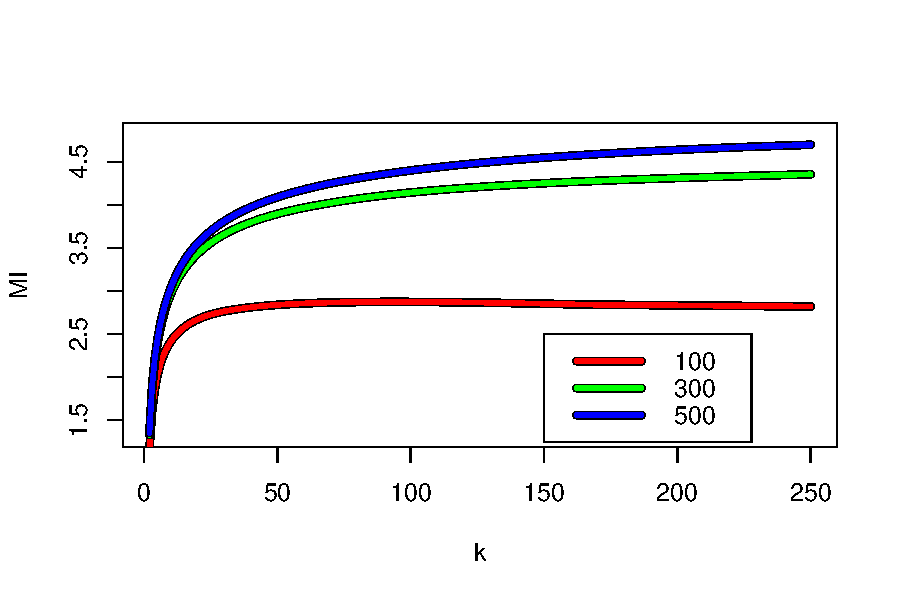
\includegraphics[scale = 0.7]{../Yuval/lower_bound.pdf}
\caption{Lower confidence bounds for $\alpha = 0.05$, for the encoding model $\vec{g}_{Gabor}$ and the subsets $S_1,S_3, S_5$.
The subset $S_i$ is the $100i$ voxels with the highest signal-to-noise
ratio.  The $x$-axis shows the $k$ used in the procedure, and the $y$
axis gives the resulting lower confidence bound
$\underline{I}(\vec{g}_{Gabor}, \Pi_S)$.}\label{fig:kaydata1}
\end{figure}




\section{Discussion}

Since the Bayes error is the large-sample limit of the achieved
classification error, a promising approach is to perform
classification using differently sized subsamples of the training
data, producing a plot of classification error versus sample size--a
``learning curve.'' One can then extrapolate the learning curve to
estimate the Bayes error (Cortes et al. 1994.) However, much work
remains to develop rigorous methodology for estimating Bayes error,
and so we leave this first issue for future work.


There is a way to improve on data-splitting, by
using \emph{cross-validation}. Essentially, one applies the
data-splitting approach multiple times, with different training and
test partitions, and aggregates the results. In principle,
cross-validation can be used to reduce the variance of the estimated
$\text{GA}$ and hence improve the power of the test.  However, since
the variance properties of cross-validation are not well-known, we
leave the examination of cross-validation to future work.

As we saw in the results section, the quality of the lower bound
$\underline{I}$ may depend on choosing the correct $k$ for the
subsampling-based lower confidence bound of $\text{ABA}_k$.  The
question of selecting an appropriate $k$ \emph{after} seeing the data
is embedded in a larger question of \emph{experimental design}.
Supposing an experiementer only has a fixed budget $N$ of
observations, which she can split into $K$ classes with $r$ repeats
each, how should she choose $K$ (and $k$) in order to get the tightest
lower confidence bound $\underline{I}(X; Y)$?  This is an issue of
practical importance for neuroimaging researchers, but again we leave
this issue for future work.

\appendix
\section{Appendix}

\begin{lemma}\label{lemma:technical1}
Let $f(t)$ be an increasing function from $[a, b] \to \mathbb{R}$, where $a < b$,
and let $g(t)$ be a bounded continuous function from $[a, b] \to \mathbb{R}$.
Define the set
\[
A = \{t: f(t) \neq g(t)\}.
\]
Then, we can write $A$ as a countable union of intervals
\[
A = \bigcup_{i=1}^\infty A_i
\]
where $A_i$ are mutually disjoint intervals, with $\inf A_i < \sup
A_i$, and for each $i$, either $f(t) > g(t)$ for all $t \in A_i$ or
$f(t) < g(t)$ for all $t \in A_i$.
\end{lemma}

\textbf{Proof of Lemma \ref{lemma:technical1}.} (This will appear in the appendix of the paper.)

The function $h(t) = f(t) - g(t)$ is measurable, since all increasing
functions are measurable.  Define $A^+ = \{t: f(t) > g(t)\}$ and $A^-
= \{t: f(t) < g(t)\}$.  Since $A^+$ and $A^-$ are measurable subsets
of $\mathbb{R}$, they both admit countable partitions consisting of open, closed, or half-open
intervals.  Let $\mathcal{H}^+$ be the collection of all partitions of $A^+$ consisting of such intervals.
There exists a least refined partition $\mathcal{A}^+$ within $\mathcal{H}^+$.
Define $\mathcal{A}^-$ analogously, and let
\[
\mathcal{A} = \mathcal{A}^+ \cup \mathcal{A}^-
\]
and enumerate the elements
\[
\mathcal{A} = \{A_i\}_{i=1}^\infty.
\]

We claim that the partitions $\mathcal{A}^+$ and $\mathcal{A}^-$ have
the the property that for all $t \in A^\pm$, ther interval
$I \in \mathcal{A}^\pm$ containing $t$ has endpoints $l \leq u$
defined by
\[
l = \inf_{x \in [a,b]} \{x: \text{Sign}(h([x, t])) = \{\text{Sign}(h(t))\} \}
\]
and
\[
u = \sup_{x \in a[,b]} \{x: \text{Sign}(h([t, x])) = \{\text{Sign}(h(t))\}\}.
\]
We prove the claim for the partition $\mathcal{A}^+$.  Take $t \in
A^+$ and define $l$ and $u$ as above.  It is clear that $(l, u) \in
A^+$, and furthermore, there is no $l' < l$ and $u' > u$ such that
$(l', x) \in A^+$ or $(x, u') \in A^+$ for any $x \in I$.  Let
$\mathcal{H}$ be any other partition of $A^+$.  Some disjoint union of
intervals $H_i \in \mathcal{H}$ necessarily covers $I$ for $i =
1,...$, and we can further require that none of the $H_i$ are disjoint
with $I$.  Since each $H_i$ has nonempty intersection with $I$, and
$I$ is an interval, this implies that $\cup_i H_i$ is also an
interval.  Let $l'' \leq u''$ be the endpoints of $\cup_i H_i$ Since
$I \subseteq \cup_i H_i$, we have $l'' \leq l \leq u \leq u''$.
However, since also $I \in A^+$, we must have $l \leq l'' \leq
u'' \leq u$.  This implies that $l''=l$ and $u''=u$.  Since $\cup_i
H_i = I$, and this holds for any $I \in \mathcal{A}^+$, we conclude
that $\mathcal{H}$ is a refinement of $\mathcal{A}^+$. The proof of
the claim for $\mathcal{A}^-$ is similar.

It remains to show that there are not isolated points in
$\mathcal{A}$, i.e. that for all $I \in \mathcal{A}$ with endpoints
$l \leq u$, we have $l < u$.  Take $I \in \mathcal{A}$ with endpoints
$l \leq u$ and let $t = \frac{l+u}{2}$.  By definition, we have
$h(t) \neq 0$.  Consider the two cases $h(t) > 0$ and $h(t) < 0$.

If $h(t) > 0$, then $t' = g^{-1}(h(t)) > t$, and for all $x \in [t,
t']$ we have $h(x) > 0$.  Therefore, it follows from definition that
$[t, t'] \in I$, and since $l \leq t < t' \leq u$, this implies that
$l < u$.  The case $h(t) < 0$ is handled similarly. $\Box$

\begin{lemma}\label{lemma:technical2}
Let $f(t)$ be a measurable function from $[a,b] \to \mathbb{R}$, where $a < b.$
Then there exists sets $\mathcal{B}_0$ and $\mathcal{B}_1$, satisfying the following properties:
\begin{itemize}
\item  $\mathcal{B} = \mathcal{B}_0 \cup \mathcal{B}_1$ is countable partition of $[a,b]$,
\item  $f(t)$ is constant on all $B \in \mathcal{B}_0$, but not constant on any proper superinterval $B' \supset B$, and
\item $B \in \mathcal{B}_1$ contains no positive-length subinterval where $f(t)$ is constant.
\end{itemize}
\end{lemma}

\textbf{Proof of Lemma \ref{lemma:technical2}.} (This will appear in the appendix of the paper.)
To construct the interval, define
\[
l(t) = \inf \{x \in [0,1]: f([x,t]) = \{f(t)\}\}
\]
\[
u(t) = \sup \{x \in [0,1]: f([t,x]) = \{f(t)\}\},
\]
Let $B_0$ be the set of all $t$ such that $l(t) < u(t)$,
and let $B_1$ be the set of all $t$ such that $l(t) = t = u(t)$.
For all $t \in B_0$, define
\[
I(t) = (l(t), u(t)) \cup \{x \in \{l(t), u(t)\}: f(x) = f(t)\}.
\]
Then we claim
\[
\mathcal{B}_0 = \{I(t): t \in B_0\}
\]
is a countable partition of $B_0$.  The claim follows since the
members of $\mathcal{B}_0$ are disjoint intervals of nonzero length,
and $B_0$ has finite length.    It follows from definition that for any $B \in B_0$, that $f$ is not
constant on any proper superinterval $B' \supset B$.

Meanwhile, let $\mathcal{B}_1$ be a countable partition of $B_1$ into
intervals.

Next, we show that for all $I \in \mathcal{B}_1$, $I$ does not contain
a subinterval $I'$ of nonzero length such that $f$ is constant on
$I'$.  Suppose to the contrary, we could find such an interval $I$ and
subinterval $I'$.  Then for any $t \in I'$, we have $t \in B_0$.
However, this implies that $t \notin B_1$, a contradiction.

Since $t \in [a,b]$ belongs to either $B_0$ or $B_1$,
letting $\mathcal{B} = \mathcal{B}_0 \cup \mathcal{B}_1$
yields the desired partition of $[a,b]$. $\Box$.

\begin{lemma}\label{lemma:mono_entropy}
Define an exponential family on $[0,1]$ by the density function
\[
q_\beta(t) = \exp[\beta t^{k-1} - \log Z(\beta)]
\]
where
\[
Z(\beta) = \int_0^1 \exp[\beta t^{k-1}] dt.
\]
Then, the negative entropy
\[
I(\beta) = \int_0^1 q_\beta(t) \log q_\beta(t) dt
\]
is decreasing in $\beta$ on the interval $(-\infty, 0]$.
and increasing on the interval $[0, \infty)$.

Furthermore, for any $\iota \in (0,\infty)$, there exist two solutions
to $I(\beta) = \iota$: one positive and one negative.
\end{lemma}

\textbf{Proof of Lemma \ref{lemma:mono_entropy}.}

Define $\beta(\mu)$ as the solution to
\[
\mu = \int_0^1 t q_\beta(t) dt.
\]
By [Wainwright and Jordan 2008], the function $\beta(\mu)$ is
well-defined.  Furthermore, since the sufficient statistic $t^{k-1}$
is increasing in $t$, it follows that $\beta(\mu)$ is increasing.

Define the negative entropy as a function of $\mu$,
\[
N(\mu) = \int_0^1 q_{\beta(\mu)}(t) \log q_{\beta(\mu)}(t) dt.
\]

By Theorem 3.4 of [Wainwright and Jordan 2008], $N(\mu)$ is convex in
$\mu$.  We claim that the derivative of $N(\mu) = 0$ at $\mu
= \frac{1}{2}$.  This implies that $N(\mu)$ is decreasing in $\mu$ for
$\mu \leq \frac{1}{2}$ and increasing for $\mu \geq \frac{1}{2}$.
Since $I(\beta(\mu)) = N(\mu)$, $\beta$ is increasing in $\mu$, and
$\beta(\frac{1}{2}) = 0$, this implies that $I(\beta)$ is decreasing
in $\beta$ for $\beta \leq 0$ and increasing for $\beta \geq 0$.

We will now prove the claim.  Write
\[
\frac{d}{d\mu} N(\mu)\bigg|_{\mu = 1/2} = \frac{d}{d\beta} I(\beta(\mu)) \bigg|_{\beta = 0} \frac{d\beta}{d\mu} \bigg|_{\mu = 1/2}.
\]
We have
\[
\frac{d}{d\beta} I(\beta) = \beta \int q_\beta t^{k-1} dt - \log Z(\beta).
\]
Meanwhile, $Z(0) = 1$ so $\log Z(0) = 0$.  Therefore,
\[
\frac{d}{d\beta} I(\beta) \bigg|_{\beta = 0} = 0.
\]
This implies that $\frac{d}{d\mu} N(\mu) |_{\mu = 1/2} = 0$, as needed.  

For the final statement of the lemma, note that $I(0) = 0$ since $q_0$ is the uniform distribution.
Meanwhile, since $q_\beta$ tends to a point mass as either $\beta \to \infty$ or $\beta \to -\infty$,
we have 
\[
\lim_{\beta \to \infty} I(\beta) = \lim_{\beta \to -\infty} I(\beta) = \infty.
\]
And, as we can check that $I(\beta)$ is continuous in $\beta$, this means that
\[
I((-\infty, 0]) = I([0,\infty)) = [0, \infty)
\]
by the mean-value theorem.  Combining this fact with the monotonicity
of $I(\beta)$ restricted to either the positive and negative half-line
yields the fact that for any $\iota > 0$, there exists $\beta_1 < 0
< \beta_2$ such that $I(\beta_1) = I(\beta_2) = \iota$.  $\Box$.

\begin{lemma}\label{lemma:variational}
For any measure $G$ on $[0, \infty]$,
let $G^k$ denote the measure defined by
\[
G^k(A) = G(A)^k,
\]
and define
\[
E[G] = \int x dG(x).
\]
\[
I[G] = \int x \log x dG(x)
\]
and
\[
\psi_k[G] = \int x d(G^k)(x).
\]
Then, defining $Q_c$ and $c_\iota$ as in Theorem 1, we have
\[
\sup_{G: E[G] = 1, I[G] \leq \iota} \psi_k[G] = \int_0^1 Q_{c_\iota}(t) t^{k-1} dt.
\]
Furthermore, the supremum is attained by a measure $G$ that has cdf
equal to $Q_c^{-1}$, and thus has a density $g$ with respect to
Lesbegue measure.
\end{lemma}

\textbf{Proof of Lemma \ref{lemma:variational}.} (This will appear in the appendix of the paper.)

Consider the quantile function $Q(t) = \inf_{x \in [0,1]}: G((-\infty,
x]) \geq t.$ $Q(t)$ must be a monotonically increasing function from
$[0,1]$ to $[0,\infty).$ Let $\mathcal{Q}$ denote the collection of
all such quantile functions.

We have
\[
E[G] = \int_0^1 Q(t) dt
\]
\[
\psi_k[G] = \int_0^1 Q(t) x^{k-1} dt.
\]
and
\[
I[G] = \int_0^1 Q(t) \log Q(t) dt.
\]

For any given $\iota$, let $P_\iota$ denote the class of probability
distributions $G$ on $[0, \infty]$ such that $E[G]=1$ and
$I[G] \leq \iota.$  From Markov's inequality, for any $G \in P_\iota$
we have
\[
G([x, \infty]) \leq x^{-1}
\]
for any $x \geq 0$, hence $P_\iota$ is tight.  From tightness, we
conclude that $P_\iota$ is closed under limits with respect to weak
convergence.  Hence, since $\psi_k$ is a continuous function, there
exists a distribution $G^* \in P_\iota$ which attains the supremum
\[\sup_{G \in P_\iota} \psi_k[G].\]
Let $\mathcal{Q}_\iota$ denote the collection of quantile functions of
distributions in $P_\iota.$ Then, $\mathcal{Q}_\iota$ consists of monotonic functions
$Q: [0,1] \to [0, \infty]$ which
satisfy
\[
E[Q] = \int_0^1 Q(t) dt = 1,
\]
and
\[
I[Q] = \int_0^1 Q(t) \log Q(t) dt \leq \iota.
\]
Let $\mathcal{Q}$ denote the collection of \emph{all} quantile functions from measures on $[0,\infty]$.
And letting $Q^*$ be the quantile function for $G^*$, we have that
$Q^*$ attains the supremum
\begin{equation}\label{eq:constrained_optim}
\sup_{Q \in \mathcal{Q}_\iota} \phi_k[Q] = \sup_{Q \in \mathcal{Q}_\iota} \int_0^1 Q(t) t^{k-1} dt.
\end{equation}
Therefore, there exist Lagrange multipliers
$\lambda \geq 0$ and $\nu \geq 0$ such that defining
\[
\mathcal{L}[Q] = -\phi_k[Q] + \lambda E[Q] + \nu I[Q]= \int_0^1 Q(t) (-t^{k-1} + \lambda + \nu \log Q(t)) dt,
\]
$Q^*$ attains the infimum of $\mathcal{L}[Q]$ over \emph{all} quantile functions,
\[
\mathcal{L}[Q^*] = \inf_{Q \in \mathcal{Q}}\mathcal{L}[Q].
\]
The global minimizer $Q^*$ is also necessarily a stationary point:
that is, for any perturbation function $\xi: [0,1] \to \mathbb{R}$
such that $Q^* + \xi \in \mathcal{Q}$, we have $\mathcal{L}[Q^*]\leq \mathcal{L}[Q^* + \xi]$.
For sufficiently small $\xi$, we have
\begin{equation}\label{eq:Lperturb}
\mathcal{L}[Q + \xi] \approx \mathcal{L}[Q] + \int_0^1 \xi(t) (-t^{k-1} + \lambda + \nu + \nu \log Q(t)) dt.
\end{equation}
Define
\begin{equation}\label{eq:nablaQ}
\nabla \mathcal{L}_{Q^*}(t) = -t^{k-1} + \lambda + \nu + \nu \log Q(t).
\end{equation}
The function $\nabla \mathcal{L}_{Q^*}(t)$ is a \emph{functional derivative} of the Lagrangian.
Note that if we were able to show that $\nabla \mathcal{L}_{Q^*}(t) = 0$,
this immediately yields
\begin{equation}\label{eq:Qstareq}
Q^*(t) = \exp[-1 -\lambda\nu^{-1} + \nu^{-1}  t^{k-1}].
\end{equation}
At this point, we know that the right-hand side of \eqref{eq:Qstareq}
gives a stationary point of $\mathcal{L}$, but we cannot be sure that
it gives the global minimzer.  The reason is because the optimization
occurs on a constrained space.  We will show that \eqref{eq:Qstareq}
indeed gives the global minimizer $Q^*$, but we do so by showing that
the set of points $t$ where $\nabla \mathcal{L}_{Q^*}(t) \neq 0$ is of
zero measure.  Since sets of zero measure don't affect the integrals
defining the optimization problem \eqref{eq:constrained_optim}, we
conclude there exists a global optimal solution with
$\nabla \mathcal{L}_{Q^*}(t) = 0$ everywhere, which is therefore given
explicitly by \eqref{eq:Qstareq} for some $\lambda \in \mathbb{R}$, $\nu \geq 0.$

We will need the following result: that for $\iota
> 0$, any solution to \eqref{eq:constrained_optim} satisfies
$\phi_k[Q] < 1$.  This follows from the fact that
\[
E[Q] - \phi_k[Q] = \int_0^1 (1-t^{k-1}) Q(t) dt,
\]
where the term $(1-t^{k-1})$ is negative, except for the one point $t
= 1$.  Therefore, in order for $\phi_k[Q] = 1 = E[Q]$, we must have
$Q(t) = 0$ for $t < 1$.  However, this yields a contradiction since
$Q(t) = 0$ for $t < 1$ implies that $E[Q] = 0$, a violation of the
hard constraint $E[Q] = 1$.

Let us establish that $\nu > 0$: in other words, the constraint $I[Q]
= \iota$ is tight.  Suppose to the contrary, that for
some $\iota > 0$, the global optimum $Q^*$ minimizes a Lagrangian with
$\nu = 0$.  Let $\phi^* = \phi_k[Q^*] < 1.$ However, if we define
$Q_\kappa(t) = I\{t \geq 1 - \frac{1}{\kappa}\} \kappa$, we have
$E[Q_\kappa] = 1$, and also for some sufficiently large $\kappa > 0$,
$\phi_k[Q_\kappa] > \phi^*$.  But since the Lagrangian lacks a term
corresponding to $I[Q]$, we conclude that $\mathcal{L}[Q_\kappa]
< \mathcal{L}[Q^*]$, a contradiction.

The rest of the proof proceeds as follows.  We will use
Lemmas \ref{lemma:technical1} and \ref{lemma:technical2} to define a
decomposition $A = D_0 \cup D_1 \cup D_2$, where $D_2$ is of measure
zero.  First, we show that assuming the existence of $t \in D_0$
yields a contradiction, and hence $D_0 = \emptyset$.  Then, again
using argument from contradiction we establish that $D_1 = \emptyset$.
Finally, since $D_2$ is a set of zero measure, this allows us to
conclude that the $Q^*(t) = 0$ on all but a set of zero measure.

We will now apply the Lemmas to obtain the necessary ingredients for
constructing the sets $D_i$.  Since $\nabla \mathcal{L}_{Q^*}(t)$ is a difference
between an increasing function and a continuous stricly increasing
function, we can apply Lemma \ref{lemma:technical1} to conclude that
there exists a countable partition $\mathcal{A}$ of the set
$A: \{t \in [0,1]: \nabla \mathcal{L}_{Q^*}(t) \neq 0\}$ into intervals such that
for all $J \in \mathcal{A}$, $|\text{Sign}(\nabla Q^*(J))| = 1$ and
$\inf J < \sup I$ .  Applying Lemma \ref{lemma:technical2} we get a
countable partition $\mathcal{B} = \mathcal{B}_0 \cup \mathcal{B}_1$
of $[0,1]$ so that each element $J \in \mathcal{B}_0$ is an interval
such that $\nabla \mathcal{L}_{Q^*}(t)$ is constant on $J$, and furthermore is not
properly contained in any interval with the same property, and each
element $J \in \mathcal{B}_1$ is an interval, such that $J$ contains
no positive-length subinterval where $\nabla \mathcal{L}_{Q^*}(t)$ is constant.
Also define $B_i$ as the union of the sets in $\mathcal{B}_i$ for $i =
0,1$.

Note that $B_0$ is necessarily a subset of $A$.  That is because if
$\nabla \mathcal{L}_{Q^*}(t) = 0$ on any interval $J$, then that $Q^*(t)$ is
necessarily not constant on the interval.  

We will construct a new countable partition of $A$, called $\mathcal{D}$.
The partition $\mathcal{D}$ is constructed by taking the union of three families of intervals,
\[
\mathcal{D} = \mathcal{D}_0 \cup \mathcal{D}_1 \cup \mathcal{D}_2.
\]
Define $D_i$ to be the union of intervals in $\mathcal{D}_i$ for $i = 0,1,2$.

Define $\mathcal{D}_0 = \mathcal{B}_0$,
Define a countable partition $\mathcal{D}_1$ by
\[
\mathcal{D}_1 = \{J \cap L: J \in \mathcal{A}, L \in \mathcal{B}_1, \text{ and } |L| > 1\},
\]
in order words, $\mathcal{D}_1$ consists of positive-length intervals where $\nabla
Q^*(t)$ is entirely positive or negative and is not constant.
Define
\[
\mathcal{D}_2 = \{J \in \mathcal{B}_1: J \subset A \text{ and } |J| = 1 \},
\]
i.e. $\mathcal{D}_2$ consists of isolated points in $A$.

One verifies that $\mathcal{D}$ is indeed a partition of $A$ by
checking that $D_0 = B_0$, $D_1 \cup D_2 = B_1 \cap A$, so that
$D_0 \cup D_2 \cup D_2 = A$: it is also easy to check that elements of
$\mathcal{D}$ are disjoint.  Furthermore, as we mentioned earlier, the
set $D_2$ is indeed of zero measure, since it consists of countably
many isolated points.

Now we will show that the existence of $t \in D_0$ implies a contradiction.
Take $t \in D$ for $D \in \mathcal{D}_0$, and let $a = \inf D$ and $b
= \sup D$.  Define
\[
\xi^+ = I\{t \in D\} (Q^*(b) - Q^*(t))
\]
and
\[
\xi^- = I\{t \in D\} (Q^*(a) - Q^*(t)).
\]
Observe that $Q + \epsilon \xi^+ \in \mathcal{Q}$ and $Q
+ \epsilon \xi^- \in \mathcal{Q}$ for any $\epsilon \in [0,1]$.  Now,
if $\nabla \mathcal{L}_{Q^*}(t)$ is strictly positive on $D$, then for some
$\epsilon > 0$ we would have $\mathcal{L}[Q^* + \epsilon \xi^-]
< \mathcal{L}[Q^*]$, a contradiction.  A similar argument with $\xi^+$
shows that $\nabla \mathcal{L}_{Q^*}(t)$ cannot be strictly negative on $D$ either.
From this pertubation argument, we conclude that $\nabla \mathcal{L}_{Q^*}(t) = 0$.
Since this argument applies for all $t \in D_0$, we conclude that $D_0
= \emptyset$: therefore, on the set $[0,1] \setminus (D_1 \cup D_2)$,
we have $\nabla \mathcal{L}_{Q^*}(t) = 0.$

The following observation is needed for the next stage of the proof.
If we look at the function $Q^*(t)$, then up so sets of neglible
measure, it is given by the expression \eqref{eq:Qstareq} on the set
$[0,1]\setminus D_1$, and it is piecewise constant in-between.  But
since \eqref{eq:Qstareq} gives a strictly increasing function, and
since $Q^*$ is increasing, this implies that $Q^*$ is discontinuous at
the boundary of $D_1$.

Now we are prepared to show that $\nabla \mathcal{L}_{Q^*}(t) = 0$ for $t \in D_1$.
Take $t \in D$ for $D \in \mathcal{D}_1$, and let $a = \inf D$ and $b
= \sup D$.  From the previous argument, there is a discontinuity at
both $a$ and $b$, so that $\lim_{u \to a^-} Q(u) < Q(t) < \lim_{u \to
b^+} Q(u)$.  Therefore, for any $\xi(t)$ which is increasing on $D$
and zero elsewhere, there exists $\epsilon > 0$ such that $\nabla Q^*
+ \epsilon \xi \in \mathcal{Q}.$ It remains to find such a
perturbation $\xi$ such that $\mathcal{L}[Q + \epsilon \xi]
< \mathcal{L}[Q]$.

Also, since by definition $\nabla \mathcal{L}_{Q^*}(t)$ is constant on $D$, follows from\eqref{eq:nablaQ} that
$\nabla Q^*$ is strictly decreasing, and thus either
\begin{itemize}
\item Case 1: $\nabla \mathcal{L}_{Q^*}(t) \geq 0$ on $D$,
\item Case 2: $\nabla \mathcal{L}_{Q^*}(t) \leq 0$ on $D$, or
\item Case 3: $\nabla \mathcal{L}_{Q^*}(t) \geq 0$ for all $t \in D \cap [a, t_0]$ and $\nabla \mathcal{L}_{Q^*}(t) \leq 0$ for all $t \in D \cap [t_0, b]$.
\end{itemize}

Depending on the case, we construct a suitable perturbation $\xi$:
\begin{itemize}
\item Case 1: Construct $\xi(t) = -I\{t \in D\}$.
\item Case 2: Construct $\xi(t) = I\{t \in D\}$
\item Case 2: Construct
\[
\xi(t) = \begin{cases}
-1 & \text{ for }t \in D \cap [a, t_0],\\
0 & \text{ otherwise. }
\end{cases}
\]
\end{itemize}
In all three cases, given the corresponding construction for $\xi(t)$ we get
\[
\int_0^1 \xi(t) \nabla \mathcal{L}_{Q^*}(t) dt < 0.
\]
Therefore, from \eqref{eq:Lperturb}, there exists some $\epsilon > 0$
such that $\mathcal{L}[Q + \epsilon \xi] < \mathcal{L}[Q]$, a
contradiction.  Again, since the contradiction applies for all $t \in
D_1$, we conclude that $D_1 = \emptyset$.

By now we have established that a global optimum
for \eqref{eq:constrained_optim} exists, and is given
by \eqref{eq:Qstareq} for some $\lambda \in \mathbb{R}$, $\nu > 0$.  It remains
to determine the values of $\lambda$ and $\nu$.

Reparameterize $\alpha = \exp[-1-\lambda\nu^{-1}]$ and $\beta = \nu^{-1}$.
Therefore,
\[
Q^*(t) = \alpha \exp[\beta t^{k-1}]
\]
for $\alpha > 0$, $\beta > 0$.  There is a one-to-one mapping from
$(\alpha, \beta) \in (0, \infty)^2$ to $(\lambda, \nu) \in
\mathbb{R} \times (0,\infty)$.

Now, from the constraint
\[
1 = E[Q^*] = \int_0^1 \alpha \exp[\beta t^{k-1}] dt.
\]
we conclude that
\[
\alpha = \frac{1}{\int_0^1 \exp[\beta t^{k-1}] dt.}
\]
Therefore, we have reduced the set of possible solutions $Q^*$ to a one-parameter family,
\[
Q^*(t) = \frac{\exp[\beta t^{k-1}]}{Z(\beta)}.
\]
where
\[
Z(\beta) = \int_0^1 \exp[\beta t^{k-1}] dt.
\]

Next, note that
\[
I[Q^*] = \int_0^1 Q^*(t) \log Q^*(t) = \beta \mu_\beta - \log Z(\beta),
\]
as a function of $\beta$, is completely characterized by Lemma \ref{lemma:mono_entropy}.
Let us define $c_\iota$ as the unique positive solution to the equation
\[
c_\iota \mu_{c_\iota} - \log Z(c_\iota) = \iota
\]
given by Lemma \ref{lemma:mono_entropy}.
We therefore have
\[
Q^*(t) = \frac{\exp[c_\iota t^{k-1}]}{\int_0^1 \exp[c_\iota t^{k-1}]},
\]
as needed. $\Box$


\begin{lemma}\label{lemma:concave}
The map
\[
\iota \to \int_0^1 Q_{c_\iota}(t) t^{k-1} dt
\]
is concave in $\iota > 0$.
\end{lemma}

\textbf{Proof of Lemma \ref{lemma:concave}.}
It is equivalent to show that the inverse function
\[
C^{-1}_k(p) = \inf_{G: E[G] = 1, \phi_k[G] = p} I[G]
\]
is convex.  Let $p_1, p_2 \in [0,1]$.  From
lemma \ref{lemma:variational}, we can find measures $G_1$, $G_2$ on
$[0,\infty)$ which minimize $I[G_i]$ subject to $E[G_i] = 1$ and
$\phi_k[G_i] = p_i$.  Define the measure
\[
H = \frac{G_1 + G_2}{2}.
\]
Since $\phi_k$ is a linear functional,
\[
\phi_k[H] = \frac{\phi_k[G_1] + \phi_k[G_2]}{2} = \frac{p_1 + p_2}{2}.
\]
But since $I$ is a convex functional,
\[
I[H] \leq \frac{I[G_1] + I[G_2]}{2}.
\]

Therefore,
\[
C^{-1}_k\left(\frac{p_1 + p_2}{2}\right) \leq I[H] = \frac{I[G_1] + I[G_2]}{2} = \frac{C^{-1}_k(p_1) + C^{-1}_k(p_2)}{2}.
\]
$\Box$.

\section{References}
\begin{itemize}
\item Gastpar, M.  Gill, P.  Huth, A.  Theunissen, F. ``Anthropic Correction of Information Estimates and Its Application to Neural Coding.'' \emph{IEEE Trans. Info. Theory}, Vol 56 No 2, 2010.
\item  A. Borst and F. E. Theunissen, ``Information theory and neural coding''
Nature Neurosci., vol. 2, pp. 947?957, Nov. 1999.
\item L. Paninski, ``Estimation of entropy and mutual information,'' Neural
Comput., vol. 15, no. 6, pp. 1191?1253, 2003.
\item I. Nelken, G. Chechik, T. D. Mrsic-Flogel, A. J. King, and J. W. H.
Schnupp, ``Encoding stimulus information by spike numbers and mean
response time in primary auditory cortex,'' J. Comput. Neurosci., vol.
19, pp. 199?221, 2005.
\item Cover and Thomas.  Elements of information theory.
\item Muirhead.  Aspects of multivariate statistical theory.
\item van der Vaart.  Asymptotic statistics.
\end{itemize}
\end{document}





